\PassOptionsToPackage{svgnames,dvipsnames,svgnames}{xcolor}
%% For double-blind review submission
\documentclass[acmsmall,review,anonymous]{acmart}\settopmatter{printfolios=true}
%% For single-blind review submission
%\documentclass[acmlarge,review]{acmart}\settopmatter{printfolios=true}
%% For final camera-ready submission
%\documentclass[acmlarge]{acmart}\settopmatter{}

%% Note: Authors migrating a paper from PACMPL format to traditional
%% SIGPLAN proceedings format should change 'acmlarge' to
%% 'sigplan,10pt'.

\bibliographystyle{ACM-Reference-Format}


%% Some recommended packages.
\usepackage{booktabs}   %% For formal tables:
                        %% http://ctan.org/pkg/booktabs
\usepackage{subcaption} %% For complex figures with subfigures/subcaptions
                        %% http://ctan.org/pkg/subcaption

%% Cyrus packages
\usepackage{microtype}
\usepackage{mdframed}
\usepackage{colortab}
\usepackage{mathpartir}
\usepackage{enumitem}
\usepackage{bbm}
\usepackage{stmaryrd}
\usepackage{mathtools}
\usepackage{leftidx}
\usepackage{todonotes}

\usepackage{listings}%
\lstloadlanguages{ML}
\lstset{tabsize=2, 
basicstyle=\footnotesize\ttfamily, 
% keywordstyle=\sffamily,
commentstyle=\itshape\ttfamily\color{gray}, 
stringstyle=\ttfamily\color{purple},
mathescape=false,escapechar=\#,
numbers=left, numberstyle=\scriptsize\color{gray}\ttfamily, language=ML, showspaces=false,showstringspaces=false,xleftmargin=15pt, 
morekeywords={string, float, int},
classoffset=0,belowskip=\smallskipamount, aboveskip=\smallskipamount
}
\let\li\lstinline


%% Joshua Dunfield macros
\def\OPTIONConf{1}%
\usepackage{joshuadunfield}


% \newtheorem{theorem}{Theorem}[chapter]
% \newtheorem{lemma}[theorem]{Lemma}
% \newtheorem{corollary}[theorem]{Corollary}
% \newtheorem{definition}[theorem]{Definition}
% \newtheorem{assumption}[theorem]{Assumption}
% \newtheorem{condition}[theorem]{Condition}


%% Listings
\makeatletter\if@ACM@journal\makeatother
%% Journal information (used by PACMPL format)
%% Supplied to authors by publisher for camera-ready submission
\acmJournal{PACMPL}
\acmVolume{1}
\acmNumber{1}
\acmArticle{1}
\acmYear{2018}
\acmMonth{1}
\acmDOI{10.1145/nnnnnnn.nnnnnnn}
\startPage{1}
\else\makeatother
%% Conference information (used by SIGPLAN proceedings format)
%% Supplied to authors by publisher for camera-ready submission
\acmConference[PL'18]{ACM SIGPLAN Conference on Programming Languages}{January 01--03, 2017}{New York, NY, USA}
\acmYear{2018}
\acmISBN{978-x-xxxx-xxxx-x/YY/MM}
\acmDOI{10.1145/nnnnnnn.nnnnnnn}
\startPage{1}
\fi


%% Copyright information
%% Supplied to authors (based on authors' rights management selection;
%% see authors.acm.org) by publisher for camera-ready submission
\setcopyright{none}             %% For review submission
%\setcopyright{acmcopyright}
%\setcopyright{acmlicensed}
%\setcopyright{rightsretained}
%\copyrightyear{2017}           %% If different from \acmYear


%% Bibliography style
\bibliographystyle{ACM-Reference-Format}
%% Citation style
%% Note: author/year citations are required for papers published as an
%% issue of PACMPL.
\citestyle{acmauthoryear}   %% For author/year citations

% !TEX root = main.tex

\newcommand{\mynote}[3]{\textcolor{#3}{\textsf{{#2}}}}
\newcommand{\rkc}[1]{\mynote{rkc}{#1}{blue}}
\newcommand{\cy}[1]{\mynote{cy}{#1}{purple}}
\newcommand{\mah}[1]{\mynote{cy}{#1}{green}}

\newcommand{\cvert}{{\,{\vert}\,}}

%% https://tex.stackexchange.com/questions/9796/how-to-add-todo-notes
\newcommand{\rkcTodo}[1]{\todo[linecolor=blue,backgroundcolor=blue!25,bordercolor=blue]{#1}}

\newcommand{\mattTodo}[1]{\todo[linecolor=green,backgroundcolor=green!2,bordercolor=green]{\tiny\textit{#1}}}
\newcommand{\mattOmit}[1]{\colorbox{yellow}{(Matt omitted stuff here)}}

%% SPACING HACKS
\def\parahead#1{\vspace{-8pt}\paragraph{{\textbf{#1}.}}}
\def\paraheadNoDot#1{\vspace{-8pt}\paragraph{{\textbf{#1}}}}
\def\subparahead#1{\vspace{-13pt}\paragraph{}\textit{#1.}}
\def\paraheadindent#1{\vspace{-13pt}\paragraph{}\textit{#1.}}
\def\paraheadindentnodot#1{\vspace{-13pt}\paragraph{}\textit{#1}}

% \newcommand{\ie}{{\emph{i.e.}}}
% \newcommand{\eg}{{\emph{e.g.}}}
% \newcommand{\etc}{{\emph{etc.}}}
% \newcommand{\cf}{{\emph{cf.}}}
% \newcommand{\etal}{{\emph{et al.}}}

%% \newcommand{\hazel}{\ensuremath{\textsc{Hazel}}}
%% \newcommand{\sns}{\ensuremath{\textsc{Sketch-n-Sketch}}}
%% \newcommand{\deuce}{\ensuremath{\textsc{Deuce}}}
\newcommand{\hazel}{\ensuremath{\textrm{Hazel}}}
\newcommand{\sns}{\ensuremath{\textrm{Sketch-n-Sketch}}}
\newcommand{\deuce}{\ensuremath{\textrm{Deuce}}}

\newcommand{\sectionDescription}[1]{\section{#1}}
\newcommand{\subsectionDescription}[1]{\subsection{#1}}
\newcommand{\subsubsectionDescription}[1]{\subsubsection{#1}}
%% \newcommand{\subsectionDescription}[1]{\subsection*{#1}}

\newcommand{\matt}{PI Hammer}
\newcommand{\ravi}{PI Chugh}
\newcommand{\cyrus}{Postdoc Omar}
%% \newcommand{\cuStudent}{CU Boulder Student}
%% \newcommand{\ucStudent}{UChicago Student}

\newcommand{\eap}{action suggestion panel\xspace}
\newcommand{\Eap}{Action suggestion panel\xspace}

\newcommand{\trackOne}{Track~1\xspace}
\newcommand{\trackTwo}{Track~2\xspace}
\newcommand{\trackThree}{Track~3\xspace}
\newcommand{\trackFour}{Track~4\xspace}
\newcommand{\subtrackOne}[1]{{#1}.1}
\newcommand{\subtrackTwo}[1]{{#1}.2}
\newcommand{\subtrackThree}[1]{{#1}.3}
\newcommand{\subtrackFour}[1]{{#1}.4}
\newcommand{\tracks}{Tracks}

\newcommand{\trackNameOne}{A Static Semantics for Typed Holes}
%% \newcommand{\trackNameOneOne}{Static Semantics for Incomplete Programs}
%% \newcommand{\trackNameOneTwo}{Dynamic Semantics for Incomplete Programs}

\newcommand{\trackNameTwo}{Live Programming with Typed Holes}

\newcommand{\trackNameThree}{Editing with Typed Holes}

\newcommand{\trackNameFour}{Direct Manipulation Programming with Typed Holes}
%% \newcommand{\trackNameFourOne}{Typed Projections}
%% \newcommand{\trackNameFourTwo}{Live Typed Projections}

%% \newcommand{\trackNameTwo}{Semantic Foundations for Transforming Incomplete Programs}
%% \newcommand{\trackNameTwoOne}{Edit Action Semantics}
%% \newcommand{\trackNameTwoTwo}{Structured Program Transformations} 

%% \newcommand{\trackNameThree}{Practical Applications of Interactive Structured Editing}
%% \newcommand{\trackNameThreeOne}{\hazel{}: A Hybrid Text and Structure Editor}
%% \newcommand{\trackNameThreeTwo}{Structured Editing in the Classroom}

\newcommand{\myfootnote}[1]{\footnote{ #1}}

\def\sectionautorefname{Section}
\def\subsectionautorefname{Section}
\def\subsubsectionautorefname{Section}

\newcommand{\code}[1]{\lstinline{#1}}

\newcommand{\codeSize}
  %% {\footnotesize}
  {\small}

%%%%%%%%%%%%%%%%%%%%%%%%%%%%%%%%%%%%%%%%%%%%%%%%%%%%%%%%%%%%%%%%%%%%%%%%%%%%%%%%
%% Spacing

\newcommand{\sep}{\hspace{0.06in}}
\newcommand{\sepPremise}{\hspace{0.20in}}
\newcommand{\hsepRule}{\hspace{0.20in}}
\newcommand{\vsepRuleHeight}{0.12in}
\newcommand{\vsepRule}{\vspace{\vsepRuleHeight}}
\newcommand{\miniSepOne}{\hspace{0.01in}}
\newcommand{\miniSepTwo}{\hspace{0.02in}}
\newcommand{\miniSepThree}{\hspace{0.03in}}
\newcommand{\miniSepFour}{\hspace{0.04in}}
\newcommand{\miniSepFive}{\hspace{0.05in}}

%%%%%%%%%%%%%%%%%%%%%%%%%%%%%%%%%%%%%%%%%%%%%%%%%%%%%%%%%%%%%%%%%%%%%%%%%%%%%%%%

% \lstset{
% %mathescape=true,basicstyle=\fontsize{8}{9}\ttfamily,
% literate={=>}{$\Rightarrow$}2
%          {<=}{$\leq$}2
%          {->}{${\rightarrow}$}1
%          {\\\\=}{\color{red}{$\lambda$}}2
%          {\\\\}{$\lambda$}2
%          {**}{$\times$}2
%          {*.}{${\color{blue}{\texttt{*.}}}$}2
%          {+.}{${\color{blue}{\texttt{+.}}}$}2
%          {<}{${\color{green}{\lhd}}$}1
%          {>?}{${\color{green}{\rhd}}$?}2
%          {<<}{${\color{green}{\blacktriangleleft}}$}1
%          {>>?}{${\color{green}{\blacktriangleright}}$?}2
%          {\{}{${\color{blue}{\{}}$}1
%          {\}}{${\color{blue}{\}}}$}1
%          {[}{${\color{purple}{[}}$}1
%          {]}{${\color{purple}{]}}$}1
%          {(}{${\color{darkgray}{\texttt{(}}}$}1
%          {)}{${\color{darkgray}{\texttt{)}}}$}1
%          {]]}{${\color{gray}{\big(}}$}1
%          {]]}{${\color{gray}{\big)}}$}1
% }

% !TEX root = hazelnut-dynamics.tex

% Violet hotdogs; highlight color helps distinguish them
\newcommand{\llparenthesiscolor}{\textcolor{violet}{\llparenthesis}}
\newcommand{\rrparenthesiscolor}{\textcolor{violet}{\rrparenthesis}}
% \newcommand{\llparenthesiscolor}{\textcolor{red}{\lfloor}}
% \newcommand{\rrparenthesiscolor}{\textcolor{red}{\rfloor}}

% HTyp and HExp
\newcommand{\hcomplete}[1]{#1~\mathsf{complete}}

% HTyp
\newcommand{\htau}{\dot{\tau}}
\newcommand{\tarr}[2]{#1 \rightarrow #2}
\newcommand{\tnum}{\texttt{num}}
\newcommand{\tehole}{\llparenthesiscolor\rrparenthesiscolor}
\newcommand{\tsum}[2]{{#1} + {#2}}

\newcommand{\tconsistent}[2]{#1 \sim #2}
\newcommand{\tinconsistent}[2]{#1 \nsim #2}

% HExp
\newcommand{\hexp}{\dot{e}}
\newcommand{\hlam}[2]{\lambda #1.#2}
\newcommand{\hap}[2]{#1(#2)}
\newcommand{\hapP}[2]{(#1)~(#2)} % Extra paren around function term
\newcommand{\hnum}[1]{\underline{#1}}
\newcommand{\hadd}[2]{#1 + #2}
\newcommand{\hehole}{\llparenthesiscolor\rrparenthesiscolor}
% \newcommand{\hhole}[1]{\setlength{\fboxsep}{0pt}\fcolorbox{red}{white}{\vphantom{)}$#1$}}
\newcommand{\hhole}[1]{\llparenthesiscolor#1\rrparenthesiscolor}
% \newcommand{\hhole}[1]{
  % \setlength{\fboxsep}{0pt}
  % \colorbox{violet!10!white!100}{\ensuremath{\llparenthesiscolor#1\rrparenthesiscolor}}}
\newcommand{\hindet}[1]{\lceil#1\rceil}
\newcommand{\hinj}[2]{\texttt{inj}_{#1}({#2})}
\newcommand{\hcase}[5]{\texttt{case}({#1},{#2}.{#3},{#4}.{#5})}

\newcommand{\hGamma}{\dot{\Gamma}}
\newcommand{\domof}[1]{\text{dom}(#1)}
\newcommand{\hsyn}[3]{#1 \vdash #2 \Rightarrow #3}
\newcommand{\hana}[3]{#1 \vdash #2 \Leftarrow #3}

% ZTyp and ZExp
\newcommand{\zlsel}[1]{{\bowtie}{#1}}
\newcommand{\zrsel}[1]{{#1}{\bowtie}}

%\newcommand{\zwsel}[1]{\adjustbox{cframe=blue}{\ensuremath{{\textcolor{blue}{\triangleright}}{#1}{\textcolor{blue}{\triangleleft}}}}}
\newcommand{\zwsel}[1]{
  \setlength{\fboxsep}{0pt}
  \colorbox{green!10!white!100}{
    \ensuremath{{{\textcolor{Green}{{\hspace{-2px}\triangleright}}}}{#1}{\textcolor{Green}{\triangleleft{\vphantom{\tehole}}}}}}
}
%\newcommand{\zwsel}[1]{{\triangleright}{#1}{\triangleleft}}

\newcommand{\removeSel}[1]{#1^{\diamond}}

% ZTyp
\newcommand{\ztau}{\hat{\tau}}

% ZExp
\newcommand{\zexp}{\hat{e}}

% Direction
\newcommand{\dParent}{\mathtt{parent}}
\newcommand{\dChild}{\mathtt{firstChild}}
\newcommand{\dNext}{\mathtt{nextSib}}
\newcommand{\dPrev}{\mathtt{prevSib}}

% Action
\newcommand{\aMove}[1]{\mathtt{move}~#1}
	\newcommand{\zrightmost}[1]{\mathsf{rightmost}(#1)}
	\newcommand{\zleftmost}[1]{\mathsf{leftmost}(#1)}
\newcommand{\aSelect}[1]{\mathtt{sel}~#1}
\newcommand{\aDel}{\mathtt{del}}
\newcommand{\aReplace}[1]{\mathtt{replace}~#1}
\newcommand{\aConstruct}[1]{\mathtt{construct}~#1}
\newcommand{\aConstructx}[1]{#1}
\newcommand{\aFinish}{\mathtt{finish}}

\newcommand{\performAna}[5]{#1 \vdash #2 \xlongrightarrow{#4} #5 \Leftarrow #3}
\newcommand{\performAnaI}[5]{#1 \vdash #2 \xlongrightarrow{#4}\hspace{-3px}{}^{*}~ #5 \Leftarrow #3}
\newcommand{\performSyn}[6]{#1 \vdash #2 \Rightarrow #3 \xlongrightarrow{#4} #5 \Rightarrow #6}
\newcommand{\performSynI}[6]{#1 \vdash #2 \Rightarrow #3 \xlongrightarrow{#4}\hspace{-3px}{}^{*}~ #5 \Rightarrow #6}
\newcommand{\performTyp}[3]{#1 \xlongrightarrow{#2} #3}
\newcommand{\performTypI}[3]{#1 \xlongrightarrow{#2}\hspace{-3px}{}^{*}~#3}

\newcommand{\performMove}[3]{#1 \xlongrightarrow{#2} #3}
\newcommand{\performDel}[2]{#1 \xlongrightarrow{\aDel} #2}

% Form
\newcommand{\farr}{\mathtt{arrow}}
\newcommand{\fnum}{\mathtt{num}}
\newcommand{\fsum}{\mathtt{sum}}

\newcommand{\fasc}{\mathtt{asc}}
\newcommand{\fvar}[1]{\mathtt{var}~#1}
\newcommand{\flam}[1]{\mathtt{lam}~#1}
\newcommand{\fap}{\mathtt{ap}}
\newcommand{\farg}{\mathtt{arg}}
\newcommand{\fnumlit}[1]{\mathtt{lit}~#1}
\newcommand{\fplus}{\mathtt{plus}}
\newcommand{\fhole}{\mathtt{hole}}
\newcommand{\fnehole}{\mathtt{nehole}}

\newcommand{\finj}[1]{\mathtt{inj}~#1}
\newcommand{\fcase}[2]{\mathtt{case}~#1~#2}

% Talk about formal rules in example
\newcommand{\refrule}[1]{\textrm{Rule~(#1)}}

\newcommand{\herase}[1]{\left|#1\right|_\textsf{erase}}

\newcommand{\arrmatch}[2]{#1 \blacktriangleright_{\rightarrow} #2}


\newcommand{\TABperformAna}[5]{#1 \vdash & #2                & \xlongrightarrow{#4} & #5 & \Leftarrow #3}
\newcommand{\TABperformSyn}[6]{#1 \vdash & #2 \Rightarrow #3 & \xlongrightarrow{#4} & #5 \Rightarrow #6}
\newcommand{\TABperformTyp}[3]{& #1 & \xlongrightarrow{#2} & #3}

\newcommand{\TABperformMove}[3]{#1 & \xlongrightarrow{#2} & #3}
\newcommand{\TABperformDel}[2]{#1 \xlongrightarrow{\aDel} #2}

\newcommand{\sumhasmatched}[2]{#1 \mathrel{\textcolor{black}{\blacktriangleright_{+}}} #2}

%%%% DYNAMICS %%%%
\newcommand{\dhexp}{\ddot{e}}

\newcommand{\expandAna}[5]{#1 \vdash #2 \leadsto #3 \Leftarrow #4 \dashv #5}
\newcommand{\expandSyn}[5]{#1 \vdash #2 \leadsto #3 \Rightarrow #4 \dashv #5}
\newcommand{\hasType}[4]{#1 \vdash #2 : #3 \dashv #4}
\newcommand{\isValue}[1]{#1~\mathsf{val}}
\newcommand{\isIndet}[1]{#1~\mathsf{indet}}
\newcommand{\stepsTo}[2]{#1 \mapsto #2}



\begin{document}

%% Title information
\title{Live Functional Programming with Typed Holes}         %% [Short Title] is optional;
                                        %% when present, will be used in
                                        %% header instead of Full Title.
% \titlenote{with title note}             %% \titlenote is optional;
                                        %% can be repeated if necessary;
                                        %% contents suppressed with 'anonymous'
% \subtitle{Subtitle}                     %% \subtitle is optional
% \subtitlenote{with subtitle note}       %% \subtitlenote is optional;
                                        %% can be repeated if necessary;
                                        %% contents suppressed with 'anonymous'


%% Author information
%% Contents and number of authors suppressed with 'anonymous'.
%% Each author should be introduced by \author, followed by
%% \authornote (optional), \orcid (optional), \affiliation, and
%% \email.
%% An author may have multiple affiliations and/or emails; repeat the
%% appropriate command.
%% Many elements are not rendered, but should be provided for metadata
%% extraction tools.

%% Author with single affiliation.
\author{First1 Last1}
\authornote{with author1 note}          %% \authornote is optional;
                                        %% can be repeated if necessary
\orcid{nnnn-nnnn-nnnn-nnnn}             %% \orcid is optional
\affiliation{
  \position{Position1}
  \department{Department1}              %% \department is recommended
  \institution{Institution1}            %% \institution is required
  \streetaddress{Street1 Address1}
  \city{City1}
  \state{State1}
  \postcode{Post-Code1}
  \country{Country1}
}
\email{first1.last1@inst1.edu}          %% \email is recommended

%% Author with two affiliations and emails.
\author{First2 Last2}
\authornote{with author2 note}          %% \authornote is optional;
                                        %% can be repeated if necessary
\orcid{nnnn-nnnn-nnnn-nnnn}             %% \orcid is optional
\affiliation{
  \position{Position2a}
  \department{Department2a}             %% \department is recommended
  \institution{Institution2a}           %% \institution is required
  \streetaddress{Street2a Address2a}
  \city{City2a}
  \state{State2a}
  \postcode{Post-Code2a}
  \country{Country2a}
}
\email{first2.last2@inst2a.com}         %% \email is recommended
\affiliation{
  \position{Position2b}
  \department{Department2b}             %% \department is recommended
  \institution{Institution2b}           %% \institution is required
  \streetaddress{Street3b Address2b}
  \city{City2b}
  \state{State2b}
  \postcode{Post-Code2b}
  \country{Country2b}
}
\email{first2.last2@inst2b.org}         %% \email is recommended


%% Paper note
%% The \thanks command may be used to create a "paper note" ---
%% similar to a title note or an author note, but not explicitly
%% associated with a particular element.  It will appear immediately
%% above the permission/copyright statement.
% \thanks{with paper note}                %% \thanks is optional
                                        %% can be repeated if necesary
                                        %% contents suppressed with 'anonymous'


%% Abstract
%% Note: \begin{abstract}...\end{abstract} environment must come
%% before \maketitle command
\begin{abstract}
\emph{Live programming environments} aim to provide programmers (and, in some cases, audiences) with continuous feedback about a program's dynamic behavior throughout the editing process. 
The problem that motivates this paper is that programming languages typically assign dynamic meaning only to programs that are syntactically well-formed and free of static type errors (collectively, \emph{complete programs}), whereas program editors frequently encounter incomplete edit states. 
Recent work by \citet{popl-paper} has made progress on the problem of working directly with incomplete programs by developing a type system for lambda terms with \emph{holes} in both expression and type position, with empty holes standing for missing expressions or types, and non-empty holes operating as ``membranes'' around type inconsistencies. 
This paper develops a corresponding dynamic semantics for incomplete functional programs. 
Rather than aborting with an exception when evaluation encounters a hole (as in  several existing systems), evaluation proceeds ``around'' expression holes, performing as much computation as is possible and tracking the dynamic environment around each hole as it flows through the program. 
These accumulated hole environments can be reported directly to the programmer by the editor as they work to fill holes. 
They also enable an ``edit-and-resume'' feature that avoids the need to restart evaluation after edits that amount to hole filling. 
Formally, our semantics combines features from gradual type theory (to handle incomplete types) and contextual modal type theory (CMTT, which provides a logical foundation for hole environment tracking) with novel structure necessary to prove key metatheoretic properties, including 1) a type safety property that accounts for expression holes (i.e. free metavariables, from the perspective of CMTT), and 2) commutativity and confluence properties that guarantee that the ``edit-and-resume'' feature is sound. 
The primary focus of this paper is on this formal development, which we have mechanized using the Agda proof assistant. 
We additionally describe a simple reference implementation, called Hazelnut Live, that exposes a language of structured edit actions that insert holes as necessary to guarantee that every edit state has some (possibly incomplete) type, based on the edit action calculus in the prior work by \citet{popl-paper}. 
Taken together, the result is a proof-of-concept live functional programming environment where dynamic feedback is truly continuous, i.e. it is available for every possible edit state. % i.e. \emph{every edit state is guaranteed to have non-trivial static and dynamic meaning}.

%In our system, evaluation treats failed casts much like it treats expression holes (rather than immediately failing with a cast error, as in gradual type theory). Prior work on contextual modal type theory did not develop an operational semantics for programs with free metavariables, which correspond to programs with holes in our formulation. 


% These incomplete edit states are sometimes transient, but at other times, they persist for extended periods of time, e.g. when the programmer is filling in the branches of a large case analysis one-by-one, or when an edit causes type errors to appear throughout a program. %This gap can cause live programming services to lag behind the programmer's edits, in many cases for an extended period of time.
\end{abstract}


%% 2012 ACM Computing Classification System (CSS) concepts
%% Generate at 'http://dl.acm.org/ccs/ccs.cfm'.
% \begin{CCSXML}
% <ccs2012>
% <concept>
% <concept_id>10011007.10011006.10011008</concept_id>
% <concept_desc>Software and its engineering~General programming languages</concept_desc>
% <concept_significance>500</concept_significance>
% </concept>
% <concept>
% <concept_id>10003456.10003457.10003521.10003525</concept_id>
% <concept_desc>Social and professional topics~History of programming languages</concept_desc>
% <concept_significance>300</concept_significance>
% </concept>
% </ccs2012>
% \end{CCSXML}

% \ccsdesc[500]{Software and its engineering~General programming languages}
% \ccsdesc[300]{Social and professional topics~History of programming languages}
%% End of generated code


%% Keywords
%% comma separated list
% \keywords{keyword1, keyword2, keyword3}  %% \keywords is optional


%% \maketitle
%% Note: \maketitle command must come after title commands, author
%% commands, abstract environment, Computing Classification System
%% environment and commands, and keywords command.
\maketitle

% !TEX root = hazelnut-dynamics.tex
\newcommand{\introSec}{Introduction}
\section{\protect\introSec} % don't like the all-caps thing that the template does, so protecting it from that
\label{sec:intro}
\cy{intro from LIVE 2017 paper is below}

Broadly speaking, live programming environments are those that granularly interleave editing and evaluation \cite{DBLP:conf/icse/Tanimoto13,DBLP:journals/vlc/Tanimoto90,McDirmid:2007:LUL:1297027.1297073,burckhardt2013s}. 
In the words of \citet{burckhardt2013s}, live programming environments 
``promise to narrow the temporal and perceptive gap 
between program development and code execution''. Examples of live programming environments include {lab notebook environments},
e.g. the popular IPython/Jupyter~\cite{PER-GRA:2007}, which allow the
programmer to interactively edit and evaluate program fragments organized into a
sequence of cells (an extension of the read-eval-print loop (REPL)); spreadsheets; {live graphics programming environments} like SuperGlue \cite{McDirmid:2007:LUL:1297027.1297073}, Sketch-n-Sketch \cite{DBLP:conf/pldi/ChughHSA16} and the tools demonstrated by Bret Victor in his lectures \cite{victor2012inventing}; the TouchDevelop live UI framework \cite{burckhardt2013s}; live mobile application development systems like Flutter \cite{flutter}; and live visual and auditory dataflow languages \cite{DBLP:conf/vl/BurnettAW98}, to name a few prominent examples.


The problem that has motivated much of our recent work is that most  
programming environments, live programming environments included,  provide feedback via various editor services only once the program being edited is syntactically well-formed and, when relevant, well-typed. This leaves a ``temporal and perceptive gap'', because programmers sometimes leave a program malformed or ill-typed for extended periods of time, e.g. as they think about what to enter at the cursor, or as they work on a different part of the program.

In view of this general problem, we recently developed a \emph{structure editor calculus} called Hazelnut where every edit state consists of a well-formed and statically meaningful, i.e. well-typed, incomplete expression, which we take to mean an expression with holes \cite{popl-paper}. This calculus addressed fundamental questions relevant to editor services that operate statically, but there was no solution in that paper to the problems faced by editor services that also require knowledge of the dynamic meaning of an incomplete program, as would be relevant to a live programming environment. For example, consider a \emph{stepper} (a.k.a. a \emph{stepwise debugger}), like that available to Haskell programmers in the GHCi system \cite{GHC-stepper} and other systems \cite{DBLP:conf/haskell/MarlowIPG07,kar13566}, to OCaml programmers with recent work on \texttt{ocamli} by \citet{ocaml-stepper} and to Standard ML programmers \cite{DBLP:journals/jfp/TolmachA95}. A stepper requires that the expression being stepped be assigned dynamic meaning according to a small-step operational semantics \cite{DBLP:journals/jlp/Plotkin04a,pfpl}, but no such semantics was defined for incomplete expressions that arise when using Hazelnut, or any of these other systems. Defining such a semantics was left as future work in the Hazelnut paper, and in a subsequent ``vision paper'' \cite{snapl17-paper}. The purpose of this paper is to sketch out our progress toward a theoretically well-grounded solution.

\matt{below are misc points that may be worth mentioning in section 1
  (somehow, somewhere), and weaving into the continuation of the story
  above:}

Type holes vs expression holes: 

The dynamics of type holes is gradual typing, including run-time cast
insertion and execution.
%
The dynamics of expression holes consists of defining
\emph{indeterminate} expressions, as placeholders for subterms that
traditionally would be deemed ``stuck'' .

In live programming, we expect that programs will generally have holes
in both terms and types (CITE?); however, to understand the mechanisms
of \HazelnutLive, it is instructive to imagine situations where the
only holes or in terms, or in types.
%
  When we only use type holes (not common in live programming, AFAIK),
  we recover gradual typing and do not need indeterminate forms
  (except for cast errors, which we classify this way).  
  % 
  When we only use expression holes, we do not need type casts, or
  the other dynamic mechanisms of gradual typing.


\cy{intro from grant section is below}

Live programming environments granularly interleave editing and evaluation,
``promis[ing] to narrow the temporal and perceptive gap 
between program development and code execution''~\cite{burckhardt2013s}.
Examples of live programming environments include {lab notebook environments},
like the popular IPython/Jupyter~\cite{PER-GRA:2007}, which allow the
programmer to interactively edit and evaluate program fragments organized into a
sequence of cells (an extension of the ubiquitous read-eval-print loop (REPL)); spreadsheets; {live graphics programming environments} like SuperGlue \cite{McDirmid:2007}, \sns{}~\cite{sns-pldi,sns-uist} and the tools demonstrated by Bret Victor in his lectures \cite{victor2012inventing}; the TouchDevelop live UI framework \cite{burckhardt2013s}; live mobile application development systems like Flutter \cite{flutter}; and live visual and auditory dataflow languages \cite{DBLP:conf/vl/BurnettAW98}, to name a few prominent examples. \cy{find somewhere to cite these tanimoto papers \cite{DBLP:conf/icse/Tanimoto13,DBLP:journals/vlc/Tanimoto90}}


Live programming environments typically cannot run incomplete programs, or they simply halt or raise an exception as soon as they encounter a hole during evaluation. This leaves a ``temporal and perceptive gap'' because the results of even those computations that do not depend critically on the hole are not available to the programmer. Our second track of research will address this gap by defining a dynamic semantics for incomplete programs that proceeds as far as possible around holes. 
Every program assigned static meaning by the semantics of Track 1 will also be assigned dynamic meaning by the semantics of Track 2.

For example, in \autoref{fig:intro-example} we saw that mapping the incomplete function \li{weighted_average} over the \li{grades} list produced an incomplete result. If holes simply raised exceptions, then the system would have aborted evaluation as soon as \li{weighted_average} was applied for the first time by \li{map}, and the programmer would not have been able to see that the result was a list of two elements, nor see the value of the sub-expression \li{10.0 *. g.hw1} for each element \li{g} of the \li{grades} list. Even programs with type inconsistencies can be evaluated under our proposed dynamics, because, as discussed in Track 1, non-empty holes operate as membranes around type inconsistencies. Taken together, the results from Tracks 1 and 2 may help to address a common complaint: that a static type discipline makes it difficult to do exploratory programming. 

Our proposed dynamics goes beyond staged evaluation (\eg{}~\cite{Taha:1999}), partial evaluation (\eg{}~\cite{Jones:1993uq}) and symbolic evaluation (\eg{}~\cite{King:1976}) in that we track the dynamic environment (\ie{}~the substitutions performed) around each instance of an expression hole in the result. This allows the programmer to see, in the sidebar of \autoref{fig:intro-example}, the actual values that the variables in scope take on everywhere that the hole they are filling ends up during evaluation. This provides a hole-oriented specification of a standard feature of debuggers: inspection of the environment at designated points in the program. Finally, this environmental information is useful (though not required) for the edit action suggestion service of Track 3 and the direct manipulation programming service of Track 4. 


% !TEX root = hazelnut-dynamics.tex
%% \newcommand{\examplesSec}{Live Functional Programming in Hazel, By Example}
%% \newcommand{\examplesSec}{Live Programming in \HazelnutLive, By Example}
\newcommand{\examplesSec}{Live Functional Programming with Typed Holes in Hazel}
\section{\protect\examplesSec} % don't like the all-caps thing that the template does, so protecting it from that
\label{sec:examples}

% !TEX root = hazelnut-dynamics.tex

\begin{figure}[t]
\begin{subfigure}[t]{\textwidth}
\centering
\includegraphics[width=0.85\textwidth,interpolate=false]{images/grades-cell-mockup.png}
\caption{Evaluating an incomplete functional program past the first hole}
\label{fig:grades-cell-mockup}
\end{subfigure}

\vspace{10px}

\begin{subfigure}[t]{\textwidth}
\centering
\includegraphics[width=0.3\textwidth,interpolate=false]{images/grades-sidebar-1.png}
~${}^\blacktriangleright$
\includegraphics[width=0.3\textwidth,interpolate=false]{images/grades-sidebar-2.png}
~${}^\blacktriangleright$
\includegraphics[width=0.3\textwidth,interpolate=false]{images/grades-sidebar-3.png}
\caption{The programming environment communicates relevant static \emph{and} dynamic information in a sidebar.}
\label{fig:grades-sidebar}
\end{subfigure}
% %% TODO once the code above is removed, scale up the screenshots
% \includegraphics[scale=0.20]{images/hazel-placeholder-0.png}

% \rkc{Draw arrows and captions on the top figure to show how to get
% to the bottom figure.
% ser navigates to hole a, types + to create a plus, types * to create a
% multiplication, types \#10 to create 10, types vh1 to create variable use.}

% \includegraphics[scale=0.20]{images/hazel-placeholder-1a.png}
\vspace{5px}

\caption{Example 1: Grades}
\label{fig:grades-example}
\vspace{-8px}
\end{figure}



\newcommand{\overviewExample}[2]{\paragraph{Example {#1}: {#2}}}

We begin with an example-driven overview of our proposed approach  within the \Hazel programming environment \citet{HazelnutSNAPL}. \Hazel is an open source web lab notebook environment based roughly on IPython/Jupyter \cite{Perez:2007:ISI:1251563.1251831}. The language of \Hazel is tracking toward parity with \Elm, a popular pure functional programming language similar to ``core ML'' \cite{czaplicki2012elm,Elm}. We assume familiarity with the basic concepts of ML/Elm (see \url{http://elm-lang.org/}).

Both the user interface and the language of \Hazel are under active development. For the sake of 
exposition, we have ``post-processed'' the examples in this section to make use of several convenient language mechanisms from \Elm~that are not yet implemented in \Hazel as of this writing. These mechanisms are orthogonal to the contributions of this paper---we have implemented all of the live programming features described in this section, both in \Hazel and in the implementation of the core calculus included in the supplement (see Sec.~\ref{sec:implementation}).

% !TEX root = hazelnut-dynamics.tex

\subsection{Example 1: Evaluating Past Holes and Hole Closures}

Consider the perspective of a teacher in the midst of developing a \Hazel{} notebook
to compute final student grades at the end of a course.
The top of \autoref{fig:grades-example} depicts the cell containing the incomplete program that 
the teacher has written so far (we omit irrelevant parts of the UI). 
%

At the top of this program, the teacher defines a
record type, \lismall{Student}, for recording a student's course data---here,
the student's name, of type
\lismall{string}, and, for simplicity, three grades, each of type \lismall{float}. The variable \lismall{students} binds a list of such student records. For simplicity, we include only three example students.
At the bottom of the program, the teacher maps a function \li{weighted_average} over this student data (\li{map} is the standard map function over lists, not shown), intending to compute a final weighted average for each student.
However, the program is incomplete because the teacher has not yet completed the body of the \lismall{weighted_average} function. This pattern is well-established: programmers often consume a function before implementing it.

Thusfar in Fig.~\ref{fig:grades-example}, the teacher has decomposed the function argument into variables by record destructuring, then multiplied the homework grade, \li{hw}, by \li{30.0} and finally inserted the \li{+} operator. The cursor now sits at an \emph{empty hole}, as indicated by the vertical bar and the green background. Each hole has a unique name (generated automatically in \Hazel), here simply \li{1}. 
%In this case, there is only one hole in the program, but in general, there may be many such holes.

Let us briefly digress: in a conventional ``batch'' programming system, writing \li{30.0*hw +} by itself would simply cause parsing to fail and there would be no static or dynamic feedback available to the programmer.
In response, the programmer might insert a temporary universal placeholder, e.g. by raising an exception as suggested in Sec.~\ref{sec:intro} (note however that Elm does not support exceptions, by design). This would cause typechecking to succeed. 
However, when the programming environment attempts to evaluate the program, 
evaluation would proceed only as far as the first \li{map} iteration, 
which would call into \li{weighted_average} and then fail when attempting to evaluate the hole.%
\footnote{In a lazy language, like Haskell, the result would be much the same because the environment forces the result for printing.}
While the stack trace would confirm that \li{weighted_average} has been called, this is not entirely satisfying.

\Hazel{} does not take this ``exceptional'' interpretation of holes. Instead, evaluation continues past the hole, treating it as an opaque expression of the appropriate type. The result, shown at the bottom of Fig.~\ref{fig:grades-cell-mockup}, is a list of length $3$, confirming that \li{map} does indeed behave as expected in this regard despite the teacher having provided an incomplete argument. Furthermore, each element of the resulting list has been evaluated as far as possible, i.e. the arithmetic expression \li{30.0*hw} has been evaluated for each corresponding value of \li{hw}, as expected. Evaluation cannot proceed any further because holes appear as addends. We say that each of these addition expressions is an \emph{indeterminate} sub-expression, and the result as a hole is therefore also indeterminate, because it is not yet a value, nor can it take a step due to holes in critical positions.

Given this indeterminate result, the teacher might take notice of the magnitude of the numbers being computed, e.g. \li{2640.0} and \li{2280.0}, and
decide immediately that a mistake has been made: the teacher wants to compute a 
weighted average between \li{0.0} and \li{100.0}, and so the correct
constant is \li{0.30} rather than \li{30.0}. (There are of course other possible fixes.)

Although these observations might 
save only a small amount of time in this case, 
% relative to the 
% situation where the teacher notices this mistake only once  
% the \li{weighted_average} function has been completed, 
it demonstrates
the broader motivations of live programming: continuous feedback about the dynamic behavior of the 
program can help confirm the mental model 
that the programmer has developed (in this case, regarding the behavior of \li{map}), or else help quickly dispel 
inconsistencies between the programmer's expectations and the 
actual behavior of the program (in this case, the arithmetic expression).

% The result itself is not the only live feedback that \Hazel reports to the programmer.
% Programmers also keep track of the names and types of the variables that are in scope at the cursor. 
\Hazel also helps programmers reason about the dynamic behavior of bound variables in scope at a hole via the \emph{live context inspector}, normally displays it as a sidebar but shown disembodied in three states in Fig.~\ref{fig:grades-sidebar}. 
In all three states, the live context inspector displays the names and types of the variables that are in scope, as is a common feature of programming environments.

New to our approach are the values associated with each binding.
These values come from the environments associated with each hole instance in the result. In this case, there are three instances of hole \li{1} in the result, numbered sequentially: \li{1:1}, \li{1:2} and \li{1:3}, arising from the three calls to \li{weighted_averages}. An environment is a partial mapping of each variable in scope to a value. We call a hole instance paired with an  environment a \emph{hole closure}, by analogy to function closures (and also due to the logical foundations detailed in Sec.~\ref{sec:calculus}). The programmer can select different closures by clicking on a hole instance (here, instance \li{1:1} was selected by default, as indicated by the purple outline), or cycle rapidly through all of the closures for the hole at the cursor by clicking the arrows, e.g. $\blacktriangleright$, at the bottom of the context inspector, or corresponding hotkeys.

\vspace{-4px}
\subsection{Example 2: Recursive Functions}\label{sec:qsort1}\label{sec:paths}
\vspace{-2px}

% !TEX root = hazelnut-dynamics.tex

\begin{figure}[t]
\begin{subfigure}[t]{\textwidth}
\centering
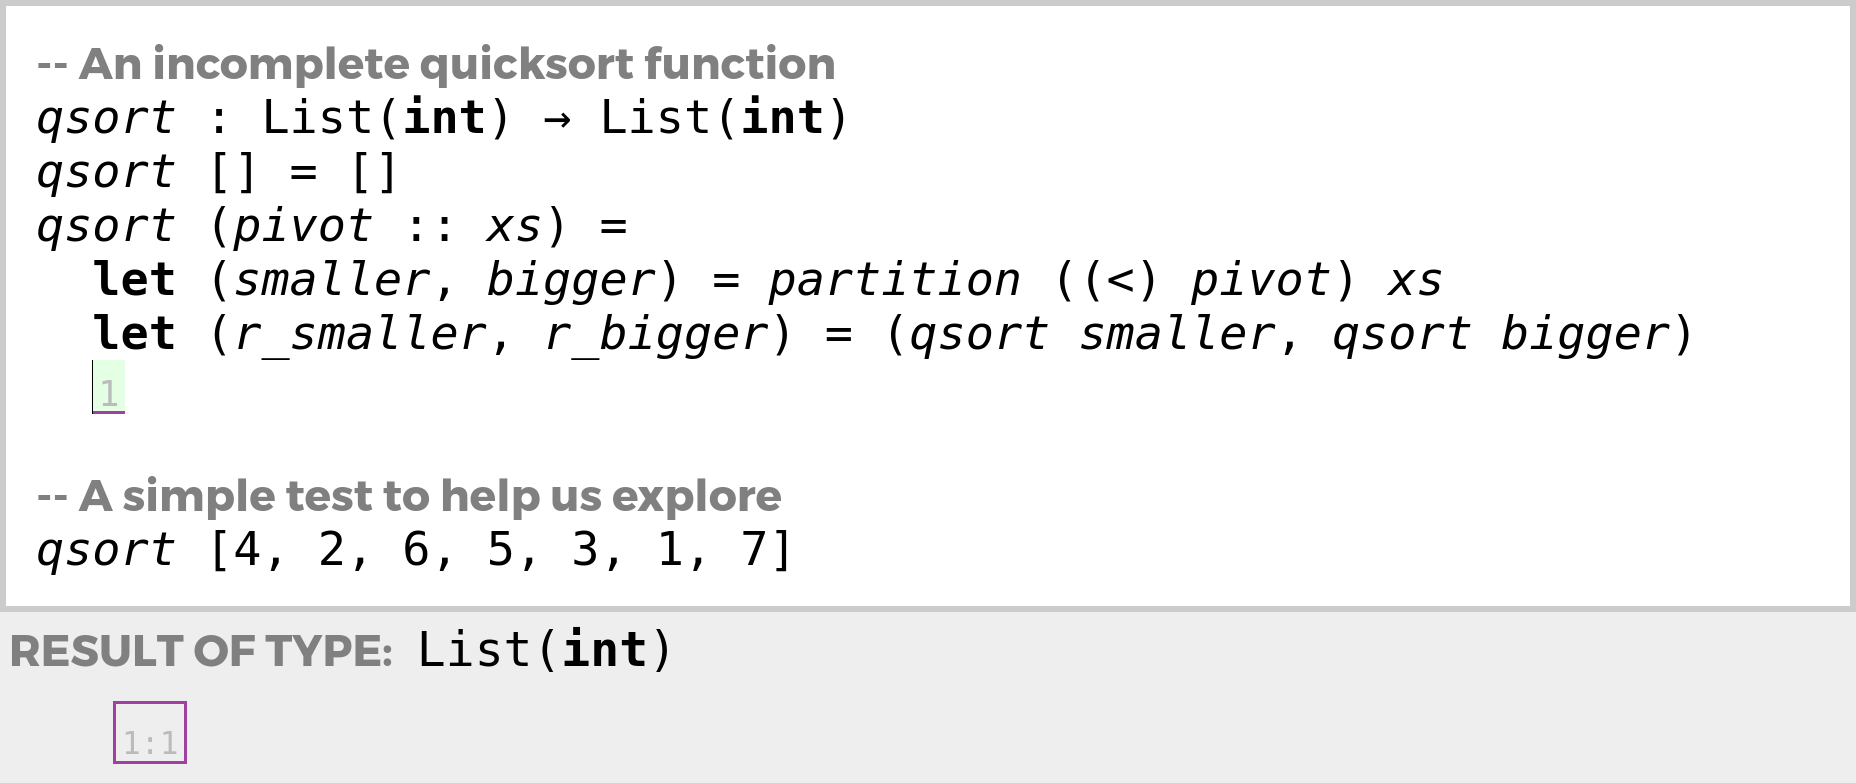
\includegraphics[width=0.57\textwidth,interpolate=false,valign=t]{images/qsort-code.png}
\vspace{-3px}
\caption{The result of evaluating this incomplete quicksort function applied to a test value is a hole closure.}
\label{fig:qsort-example-code}
\end{subfigure}

\vspace{10px}

\begin{subfigure}[t]{\textwidth}
\centering
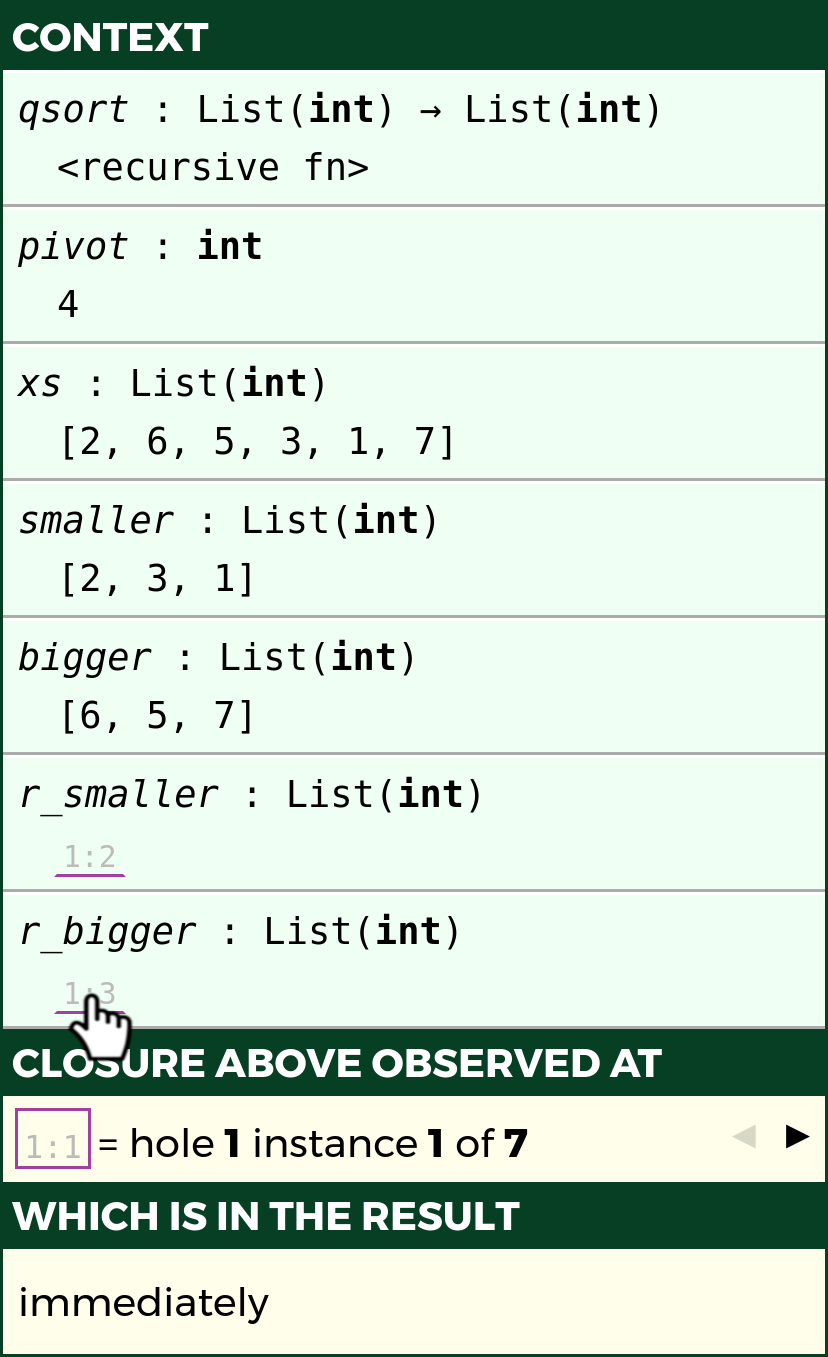
\includegraphics[width=0.29\textwidth,interpolate=false,valign=c]{images/qsort-new-sidebar-1.png}
~$\xrightarrow[\text{click}]{}$
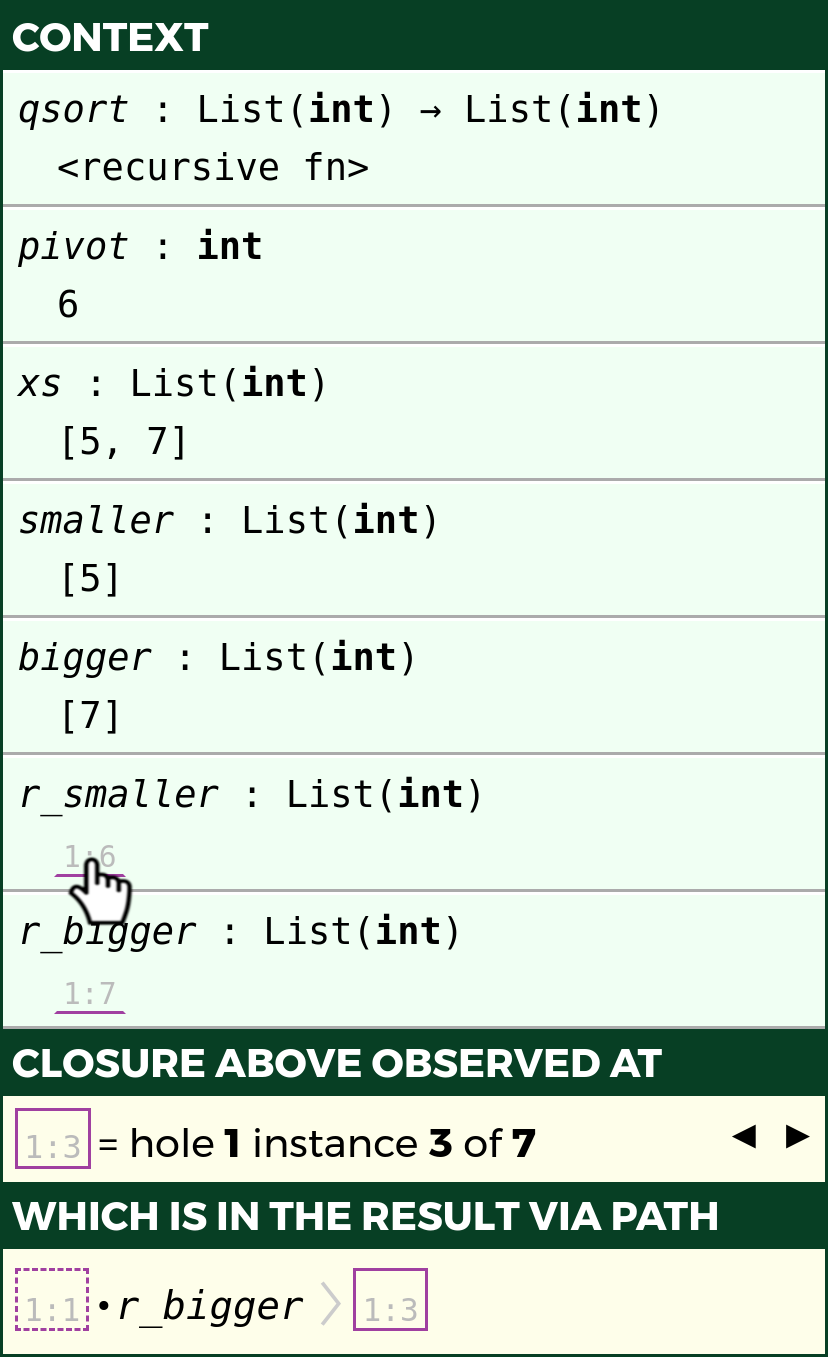
\includegraphics[width=0.29\textwidth,interpolate=false,valign=c]{images/qsort-new-sidebar-2.png}
~$\xrightarrow[\text{click}]{}$
\includegraphics[width=0.29\textwidth,interpolate=false,valign=c]{images/qsort-new-sidebar-3.png}
\caption{The programmer can explore the recursive structure of the computation by clicking on hole instances.}
\label{fig:qsort-sidebars}
\end{subfigure}

\vspace{3px}

\caption{Example 2: Incomplete Quicksort}
\label{fig:qsort-cell-mockup}
% \end{subfigure}
\end{figure}

% \begin{subfigure}[t]{\textwidth}
% \centering
% \includegraphics[width=0.3\textwidth,interpolate=false]{images/grades-sidebar-1.png}
% ~${}^\blacktriangleright$
% \includegraphics[width=0.3\textwidth,interpolate=false]{images/grades-sidebar-2.png}
% ~${}^\blacktriangleright$
% \includegraphics[width=0.3\textwidth,interpolate=false]{images/grades-sidebar-3.png}
% \caption{Typing context view with live hole closure information}
% \label{sec:grades-sidebar}
% \end{subfigure}
% %% TODO once the code above is removed, scale up the screenshots
% \includegraphics[scale=0.20]{images/hazel-placeholder-0.png}

% \rkc{Draw arrows and captions on the top figure to show how to get
% to the bottom figure.
% ser navigates to hole a, types + to create a plus, types * to create a
% multiplication, types \#10 to create 10, types vh1 to create variable use.}

% \includegraphics[scale=0.20]{images/hazel-placeholder-1a.png}


The first example was purposely simple. Let us briefly consider a second more sophisticated example of these concepts: an incomplete implementation of quicksort as a recursive function, shown in Fig.~\ref{fig:qsort-cell-mockup}. Here, the programmer has selected a pivot, split the remainder of the list relative to this pivot and made the appropriate recursive calls. A hole appears in the return position of the function body as the programmer contemplates how to combine the results from the recursive calls. 

The programmer has called \li{qsort} on an example list. However, 
the indeterminate result in this case is rather uninteresting: it simply confirms that for this example, evaluation went through the recursive case of \li{qsort}, which ends with hole \li{1}. The live context inspector, on the other hand, provides a wealth of feedback about the dynamic behavior of this incomplete program. For example, the programmer can confirm that
the lists \li{smaller} and \li{bigger} are appropriately named.

The results from the recursive calls, \li{r_smaller} and \li{r_bigger}, are again hole instances, \li{1:2} and \li{1:3}. The programmer can click on these hole instances to reveal the environments at the corresponding recursive calls. For example, clicking on \li{1:2} reveals that the pivot in that case is \li{7} (not shown). In exploring these paths rooted at the result, the programmer can develop intuitions about the recursive structure of the computation before the program is complete. 
(We leave to future work the pedagogical question of whether such early feedback might help students with recursion.)


\begin{comment}
Now the teacher returns to \lismall{weighted_average} to work on the missing
expression, with the goal of computing a weighted sum of each of a student's
grades.
%
The teacher performs several \Hazel{} edit actions (each of which is a single
keystroke, a shortcut to selecting one of the edit tools from the left panel,
followed by a tool-specific argument terminated with the Enter key):
%
navigating the cursor to hole \lismall{a} and typing \lismall{+}, which creates a
sum expression \lismall{??_b + ??_c} with the cursor placed, by default, under
left operand (the hole labeled \lismall{b});
%
typing \lismall{*} to create a multiplication expression \lismall{??_d * ??_e + ??_c},
with the cursor place under hole \lismall{d};
%
typing \lismall{\#10} to enter a numeric scaling factor, which then moves
the cursor to the second operand, hole \lismall{e}; and
%
typing \lismall{vg.hw1} to use the \lismall{hw1} field of the function argument
as the right operand of the multiplication.
%
The resulting partial expression, \lismall{(10.0 *. g.hw1) +. ??_b}---shown
in the screenshot in the bottom half of \autoref{fig:grades-example}---marks the
first of five weighted summands in the eventual finished \lismall{weighted_average}
calculation.
\end{comment}

\begin{comment}
Each \Hazel{} edit action transforms an incomplete but well-formed and
well-typed program into another such program, and, thus, \Hazel{} immediately
runs the program after each edit.
%
After the above edit sequence, \Hazel{} display the updated list of
indeterminate expressions \lismall{[760.0 + ??_b.1, 880.0 + ??_b.2, ...]}.
%
Right away, the teacher recognizes that the values are too large; they should be
at most \lismall{100.0}.
%
The teacher realizes that representing percentage points as \lismall{float}s requires
that the constant on line \rkc{XXX} ought to be \lismall{0.10} instead.
%
Because of this live feedback, the teacher corrects this error right away and
avoids making similar programming errors in the rest of the calculation.
%
The teacher continues to build the rest of the arithmetic expression until it is
complete (there are no longer any expression holes), and the result of
immediately running the finished program shows that each of values in the final
result list is in the range \lismall{0.0} to \lismall{100.0}.
\end{comment}

\begin{comment}
\begin{figure}[t]

\rkc{Move all this code into the mockup screenshots below.}

\lstset{basicstyle=\scriptsize\ttfamily}
\begin{lstlisting}
type grade_cutoffs =
  { a: float, b: float, c: float, d: float, f: float };

let cutoffs =
  { a = ??_a, b = ??_b, c = ??_c, d = ??_d, f = ??_f };

let letter_grade(n: weighted_average) =
  if n >= cutoffs.a then "A" else
  if n >= cutoffs.b then "B" else
  if n >= cutoffs.c then "C" else
  if n >= cutoffs.d then "D" else
  if n >= cutoffs.f then "F" else "Incomplete";

let sorted_weighted_averages = List.sort weighted_averages;

let letter_grades = List.map letter_grade sorted_weighted_averages;

let compute_distribution(list: list(float)) =
  let n = List.length letter_grades in
  List.map
    (\x -> (x, showPercentage (List.length (List.filter ((==) x) list)) /. n))
    ["A","B","C","D","F","Incomplete"];

let distribution = compute_distribution(letter_grades);
\end{lstlisting}
%% restore settings from main.tex
\lstset{basicstyle=\footnotesize\ttfamily}

\includegraphics[scale=0.27]{images/hazel-placeholder-1b.png}

\caption{Hazel mockup for Example 1b.}
\label{fig:grades-example-b}
\end{figure}


\overviewExample{1b}{Assigning Letter Grades}
%
The teacher's next task is to map the weighted averages to the letter grades A
through F (we consider only ``whole'' letter grades, for simplicity).
%
The \lismall{grade_cutoffs} record type, shown at the top of
\autoref{fig:grades-example-b}, describes the minimum cutoff for each of
these six possible grades.
%
Initially, each value in the \lismall{cutoffs} record is a hole.

%
%% initially all holes, because it will be different year-to-year based on the %
%data, differences in course difficulty, and to satisfy fairness criteria.
%
Before starting to fill in the cutoff values, the teacher jumps ahead to write a
function \lismall{letter_grade} that will make the connection between \lismall{cutoffs}
and \lismall{weighted_averages}.
%
Because she intends to look at the data to help select the cutoff values, the
teacher sorts the \lismall{weighted_averages} (on line \rkc{XXX}) and then maps
them to \lismall{letter_grades} (on line \rkc{XXX}).

When \Hazel{} runs this program, the guard of the outermost conditional
(\lismall{n >= cutoffs.a} on line \rkc{XXX}), is indeterminate because \lismall{cutoffs.a}
is.
%
Therefore, each of the indeterminate expressions in \lismall{letter_grades} is the
entire expression body, albeit with different bindings for \lismall{n}.
%
Displaying such ``large'' indeterminate expressions can quickly consume all
available screen space, overwhelming the user with too much information.
%
\autoref{fig:XXX} shows how \Hazel{} renders large indeterminate
expressions (\ie{}~anything other than ``small'' indeterminate value (a constant
or hole) or list of small values) simply as \lismall{..} to save space.
%
Hovering over this abbreviation (\rkc{???}) displays the full
indeterminate expression---as well as the evaluation environment that surrounds
it---as a tooltip.
%
\autoref{sec:discussion} discusses this and other user interface concerns when
trying to display useful live feedback without overwhelming the user.
%
These usability factors are beyond the scope of our work, which is to define
semantic foundations on which such user interfaces can be built.

To start deciding \lismall{cutoffs}, the teacher clicks the \lismall{weighted_averages}
expression, and views the results panel to see the data sorted in descending
order.
%
The result shows a natural gap between \lismall{92.2} and \lismall{89.5}.
%
So, she chooses to use \lismall{92.0} as the cutoff for A, replacing hole \lismall{XXX} on
line \rkc{XXX} with that numeric value.
%
Resuming the computation from before, \Hazel{} resolves the conditional
expressions for the first \rkc{XXX} indeterminate expressions, because each of
those \lismall{n} values was greater than \lismall{cutoffs.a}.
%
The remaining \rkc{XXX} expressions also proceeded to evaluate the first guard,
and are now indeterminate at the guard for the second conditional.

Before assigning subsequent cutoff values, the teacher would like to get a sense
of whether this first choice is a good one.
%
She jumps ahead to to write a function (\lismall{compute_distribution} on lines
rkc{XXX}-\rkc{XXX}) that computes the distribution of letter grades based
on \verb+cutoffs+..
%
Running \lismall{compute_distribution} shows that the percentage of As is
\rkc{XXX\%}, which is smaller than what the teacher would like;
the remaining percentages are all indeterminate.
%
Returning to the value of \lismall{sorted_data}, she sees a cluster around \lismall{89.0}
and then another gap between \lismall{88.2} and {85.5}.
%
So, the teacher adjusts \lismall{cutoffs.a} to be \lismall{88.0}.
%
Because this edit is not just filling a hole expression, \Hazel{} discards the
previous execution state and reevaluates the entire program.
%
Existing techniques for incremental computation~\cite{XXX,XXX}, however, could
be applied to seek opportunities for reuse even when non-hole expressions are
modified.
%
Because the focus of work is on the novel implications of running programs with
holes, our calculus and implementation supports caching ``edit-and-resume'' only
for the novel situation in which evaluation proceeds around holes.
%
After re-evaluation, the percentage of As becomes \rkc{XXX\%}, which better
matches the teacher's intention.

In this fashion, the teacher continues down the list of sorted averages,
determining appropriate values for each cutoff.
%
Whenever the teacher is only filling in the ``next'' cutoff, the computation
from before can simply be resumed.
%
Overall, throughout the workflow described in these two examples, the programmer
can continue to evaluate the program, and receive meaningful feedback, while
going back and forth between different pieces under development.
\end{comment}

% !TEX root = hazelnut-dynamics.tex

%% \subsection{Live Programming with Type Errors}

\subsection{Example 3: Live Programming with Static Type Errors}
\label{sec:static-errors}


% \begin{subfigure}[t]{\textwidth}
\begin{figure}
\centering
\includegraphics[width=0.7\textwidth,interpolate=false,valign=t]{images/qsort-type-error.png}
\caption{Example 3: Ill-Typed Quicksort}
\label{fig:qsort-type-error}
\vspace{-8px}
\end{figure}
% \end{subfigure}


The previous examples were incomplete 
because of \emph{missing} expressions.
%
Now, we discuss programs that are incomplete, 
and therefore conventionally meaningless, because of
\emph{type inconsistencies}. 
%
Let us return to the quicksort example just described, 
but assume that the programmer has filled in the previous hole
as shown in Fig.~\ref{fig:qsort-type-error}. (In Sec.~\ref{sec:resumption}, we discuss
how the programming environment might avoid restarting evaluation after such edits, but for small examples like this, restarting works fine.)

The programmer appears to be on the right track conceptually
in recognizing that the pivot needs to appear between the 
smaller and bigger elements. 
However, the types do not quite work out: the \li{@} operator here
performs list concatenation, but the pivot is an integer. 
Most compilers and editors will report a static error message, 
of varying utility, to the programmer in this case (and \Hazel 
follows suit, not shown). 
Our argument is that this should not cause all feedback about 
the dynamic behavior of the program to ``flicker out'' or ``go stale''. After all,
the error is localized and there is perfectly good code elsewhere 
in the program (if not nearby, then perhaps far away).

Our approach, following the prior work of \citet{popl-paper}, 
is to semantically internalize the ``red outline'' around
type inconsistencies as a \emph{non-empty hole}.
From the outside, a non-empty hole behaves statically much like an empty hole.
Our approach takes the same approach for the dynamic semantics,
i.e. evaluation safely proceeds past a non-empty hole just as if it were an empty hole.
The semantics also associates an environment with each instance of a non-empty hole (not shown). 
The difference is that evaluation also proceeds inside the hole, so that 
feedback about an expression that might ``almost'' be correct is available. 
In this case, the result at the bottom of Fig.~\ref{fig:qsort-type-error}
reveals that the programmer is on the right track: the list elements 
(here, for a shorter example for the sake of exposition) are in the right order.
They simply have not been combined correctly.

% For example, consider the following two definitions.

% \begin{lstlisting}
% let bad_bool : bool = ?? 0 ??_bad_bool;

% let bad_int : int = 1 + ?? true ??_bad_int_second_argument;
% \end{lstlisting}

% \noindent
% %
% These two definitions are ill-typed under standard typing disciplines.
% %
% In contrast, \citet{popl-paper} present a bidirectional type system that assigns
% types to both, by wrapping type-inconsistent expressions (\li{0} on line
% \rkc{XXX} and \li{true} on line \rkc{XXX} above) in \emph{non-empty} holes.
% %
% Non-empty holes prevent local type inconsistencies from polluting the rest of
% the program surrounding it, which may or may not itself contain additional
% inconsistencies.

\begin{comment}
\overviewExample{2}{Sum List}
%
Consider the following buggy program (observed during an undergraduate
functional programming course~\cite{Seidel2016}) that attempts to sum a list
integers.
%
The error is that the base case produces a list rather than an integer.

\begin{lstlisting}
sum_list : list(int) -> int
sum_list [] = ?[]?
sum_list (n:ns) = n + sum_list ns
\end{lstlisting}

\noindent
%
Because the list expression on line 2 does not have type \li{int} as required,
it is wrapped in a (non-empty) hole by the bidirectional type
checker~\cite{popl-paper}.
%
Rather than trying to debug the error based on the static error, the programmer
may wish to trying running the function anyway by calling, say, \li{sum_list(2)}.
%
\HazelnutLive{} runs and produces the indeterminate expression \li{3 + ?[]?}.
%
By observing that the hole expression is being added to the integer \li{3}, he
realizes that it needs to be an integer, specifically, \li{0}.
%
Compared to the trace displayed by \citet{Seidel2016}, the indeterminate result
produced by \HazelnutLive{} is ``flattened'' because the expression \li{1 + 2}
successfully proceeded to evaluate despite the error elsewhere.
\end{comment}

%% TODO fold error from Erwig paper.
%% %
%% see that final call on stack does have the right answer, but
%% it's wrapped in a singleton list when the expected type is not
%% a list.
%% %
%% fix is to remove the list, the rest of the computation remains
%% the same, but b/c they were all wrapped in holes, need to re-run.
%% %
%% (add some mechanism for type-consistent non-empty-holes...)

\begin{comment}

\overviewExample{4}{Stutter}
%
Consider the following function which attempts to produce a
list where every element is repeated twice (borrowed from \citet{Osera2015}).
%
The combiner function to \li{List.foldr} needs to produce a \li{list(int)}, but
it produces a \li{list(list(int)} instead.

\begin{lstlisting}
stutter : list(int) -> list(int)
stutter xs = List.foldr (\x acc -> ?[x,x]? : acc) [] xs
\end{lstlisting}

\noindent
%
The bidirectional type checker of \citet{popl-paper} wraps the expression
\li{[x,x]} inside a non-empty hole.
%
%% The editor has a choice about which expression to ``blame'' for the error; the
%% entire application that forms the body of the lambda is analyzed against the
%% return type \li{list(int)}, so that is a reasonable choice for the editor to
%% make; another would be to assume that the arguments \li{[x,x]} and \li{acc} are
%% both as intended and that only the function \li{(:)} is type-consistent.
%% %
%% Although one could imagine a setting in which a user would perform this
%% reasoning, let's assume the simplest approach for marking consistencies that
%% wraps the entire application.
%
Running this on \li{stutter [1,2,3]} produces the indeterminate result

\begin{lstlisting}
?  [1,1] : (? [2,2] : (? [[3:3]] ?) ?) ?,
\end{lstlisting}

\noindent
%
which shows the unfolding of \li{List.foldr}.
%
We refer to nested indeterminate computations like this as \rkc{\emph{hole
environment traces} or \emph{hole environment trees}}.
%
The result of the innermost indeterminate expression is \li{[[3,3]]}.
%
The user realizes that there are too many levels of nesting, so
he replaces the \li{(:)} with \li{(@)}, which addresses the type inconsistency
and, when reevaluated, produces the desired result.

\end{comment}

% !TEX root = hazelnut-dynamics.tex

\vspace{-4px}
\subsection{Example 4: Dynamic Type Errors}
\label{sec:dynamic-type-errors}
\vspace{-2px}
So far, we have only discussed programs where a hole appears within an expression.
\Hazel also allows holes to appear in types.
Fortunately, \citet{popl-paper} confirms that the substantial literature on \emph{gradual type systems} \cite{Siek06a,DBLP:conf/snapl/SiekVCB15} is directly relevant to the problem of reasoning statically around type holes.
Unsurprisingly, it is also relevant to the problem of running 
programs with incomplete types. Indeed, that is the very purpose of gradual typing. As such, let us consider only a small synthetic example to demonstrate what is different in \Hazel.
\begin{lstlisting}
f : ? -> int
f x = if x then 1 else 2
(f true, f 3, f false)
\end{lstlisting}
Evaluation produces the following result:
\begin{lstlisting}[numbers=none]
(1, if SSTR3<int => ? =/> bool>ESTR then 1 else 2, 2)
\end{lstlisting}
Here, we have left a hole, \li{?}, in the type of \li{f}. On Line 3, we call \li{f} three times, with two different types of arguments. The static semantics of gradual typing permits all of these calls (see next section) and indeed, the first call, with \li{true} as the argument, evaluates unproblematically to \li{1}. 

The second call, however, is problematic: \li{3} is of type \li{int} but it flows into boolean guard position. The usual semantics for gradual typing would simply abort evaluation here with a dynamic type error. However, this deprives the programmer of live feedback about other parts of the program that might not depend at all on this problematic function call---in this case, the third call to \li{f}. Instead, we follow the approach we took above for static type inconsistencies: we treat a failed cast like a hole. A failed cast, notated textually and in red \li{SSTR3<int => ? =/> bool>ESTR} (see next section), reports both the expected type, here \li{bool}, and the assigned type, here \li{int}. Consequently, the second call to \li{f} stops as if the guard were an empty hole, but the third call can progress safely.

\begin{comment}
\emph{Gradual type systems}~(\eg{}~\cite{XXX,XXX,XXX}) can statically accept
programs that would otherwise be rejected by static type systems---either
because type inference cannot reconstruct a valid type assignment, or because
there may not be a unique valid type assignment at all.
%
In either case, gradual type systems allow types to contain \emph{unknown
types}, and partially unknown types can be used in contexts that require
different types, so long as they are \emph{consistent} (intuitively, equal
modulo the unknown parts).
%
Dynamic casts are then inserted to ensure that these remaining static
discrepancies are not violated at run-time.

\HazelnutLive{} inherits the notion of \emph{type holes} from
\citet{popl-paper}, which serves a similar static purpose as the unknown type in
gradual type systems.
%
In contrast to prior gradually typed languages, however, \HazelnutLive{} can
evaluate ``around'' cast errors in the same way as it does for expression holes.

\overviewExample{3}{Dynamically Typed Negation}

Consider the \li{negate} function (adapted from \cite{ChughPOPL2012}), which
cannot be assigned a static type in a conventional type system---either a
bidirectional one, like in \HazelnutLive{}, or one with ML-style,
unification-based inference---because the argument \li{x} is used at type
\li{int} on line \rkc{XXX} and \li{bool} on line \rkc{XXX}.
%
Therefore, the declared type of \li{x} is the hole type \li{??}, which allows
\li{x} to be used at the conflicting types, with each use expanded into an
expression wrapped in a \emph{cast} that will dynamically check for safety.
%
The return type also uses the hole type \li{??}, leading to additional casts in
the expansion.

\begin{lstlisting}
negate : bool -> ?? -> ??
negate b x =
  if b
    then 0 - x     // expanded to: (0 - (x<?? => int>))<int => ??>
    else not x     // expanded to: (not (x<?? => bool>))<bool => ??>

(negate false 1) + 2 + 3 + (negate true 4)
\end{lstlisting}

\noindent
%
As in prior gradually typed languages~\cite{XXX},
evaluating the expression \li{negate false 1} on line \rkc{XXX} leads to
\li{(not (1<int => ??><?? => bool>))<bool => ??>}, where the inner casts
lead to the \emph{cast error} \li{1<?? =/=> bool>} because \li{1} cannot be
safely treated as having type \li{bool}.
%
Unlike in prior gradually typed languages, however, \HazelnutLive{} evaluates
around the cast error, making progress on the \li{2 + 3 + negate false 4}
expression that surrounds the error; the final indeterminate result is
\li{(not (1<?? =/=> bool>))<bool => ??> + 1}.
%
Just like it is useful for static type checkers to report multiple errors, our
approach allows us to report multiple dynamic cast errors, and otherwise make
progress on expressions that do not depend on failed casts.
%
This approach can be incorporated into existing gradually typed languages.
\end{comment}
\subsection{Live Programming for Debugging}

Previous examples highlighted how running different kinds of incomplete
programs---ones with missing expressions, type-inconsistent expressions, or
missing types---can be useful.
%
Our final example demonstrates how expression holes may be useful even for
complete programs, in order to facilitate debugging and program understanding.

%% \overviewExample{6}{\rkc{...}}
%%
%% \rkc{breakpoints, understanding input/output behavior}

\overviewExample{6}{Quicksort}

Consider the following buggy implementation of quicksort, which contains several
errors.
%
The student wants to debug the implementation and so inserts an expression
around the return expression on line \rkc{XXX}, and runs
\li{quicksort [X,X,X,X,X,X]}.

\begin{lstlisting}
quicksort : list('a) -> list('a)
quicksort [] = []
quicksort (x:xs) =
  let (left, right) = span ((>) x) xs in
  let (left', right') = (quicksort left, quicksort right) in
  ? (left' @ [x] @ right) ?
\end{lstlisting}

\noindent
%
Based on the live environment for the initial call, the student notices that the
values in \li{left} are larger than the pivot \li{x}, but \li{left} was intended
to bind smaller values.
%
This suggests that the student got the filtering predicate backwards, so he
replaces it with \li{(<)} on line \rkc{XXX}.
%
After re-running the program and viewing the live output again, \li{left} now
contains smaller values than \li{x}, but not all of them; \li{right} has some
values that are larger and some that are smaller.
%
The student uses type-based search to find other functions, besides \li{span},
of type \li{('a -> bool) -> 'a list -> ('a list, 'a list)} and finds
\li{partition}.
%
It may be easier for the student to simply try the function rather than studying
the documentation, so he edits line \rkc{XXX} to call \li{partition} instead,
re-runs, and observes that both \li{left} and \li{right} now seem to achieve the
intended partitioning.

Despite these two fixes, the result expression is not yet sorted.
%
In particular, the values greater than the pivot \li{x} are not completely
sorted.
%
Viewing the values of bindings of \li{left'} and \li{right'}, the student sees
that both seem to have correct prefixes of sorted lists, but that they are
incorrect after the pivots.
%
This suggests that something may be wrong with the handling of \li{right'}.
%
Indeed, the student takes a look for uses of \li{right'} and sees that line
\rkc{XXX} mistakenly uses \li{right} instead.
%
Making this change and re-running now produces the desired result, built up as a
hole environment tree that shows how all of the recursive results will be
combined by a series of nested appends.
%
Happy with the results of the program, the student removes the hole around the
expression on line \rkc{XXX}, and evaluation can proceed to perform the nested
appends, producing the final sorted result.
%
\autoref{sec:discussion} discusses how debugging tools may be designed to
systematically insert hole expressions in particular places to achieve certain
debugging and program understanding strategies.
%
%% When run on a larger input, this projection of the full evaluation trace shows a
%% nesting structure---which could be rendered as visualization to help
%% understanding, as described in \autoref{sec:discussion}---whose depth is clearly
%% much smaller than the length of the input list; this suggests that the
%% algorithm, indeed, achieves some sort of sublinear complexity, as intended.
%

\begin{lstlisting}
quicksort : list('a) -> list('a)
quicksort [] = []
quicksort (x:xs) =
  let (left, right) = partition ((<) x) xs in
  let (left', right') = (quicksort left, quicksort right) in
  ? (left' @ [x] @ right') ?
\end{lstlisting}



% \paragraph{Recap}
% %
% In the above four subsections, respectively, we considered programs with:
% %
% (1) empty expression holes,
% %
% (2) non-empty expression holes for ill-typed expressions,
% %
% (3) type holes, and
% %
% (4) non-empty expression holes for well-typed expressions.
% %
% Next, we will formally describe the novel dynamic semantics of \HazelnutLive{}
% that allows programs with combinations of these kinds of incompleteness to be
% evaluated.

% !TEX root = hazelnut-dynamics.tex

\clearpage
\newcommand{\calculusSec}{Hazelnut Live, Formally}
\section{\protect\calculusSec}
\label{sec:calculus}

We will now make the intuitions developed in the previous section formally precise by specifying the \HazelnutLive core calculus and  its accompanying metatheory. We have mechanized these formal developments using the Agda proof assistant \cite{norell:thesis,norell2009dependently} (see Sec.~\ref{sec:agda-mechanization} for some additional details and the supplemental material for the full mechanization). % The proofs of the metatheorems are established by this mechanization; the proofs are only very briefly outlined in this section.

The syntax of the core calculus, specified in Fig.~\ref{fig:hazelnut-live-syntax}, consists of types and expressions with holes. We distinguish between \emph{external} expressions, $e$, and \emph{internal} expressions, $d$. External expressions correspond to programs as entered by the programmer (see Sec.~\ref{sec:implementation}\todo{or maybe Sec. 2?}{} for discussion of manual, semi-automated and fully automated hole entry methods). Each well-typed external expression (as specified in Sec.~\ref{sec:external-statics} below) expands to a well-typed internal expression (see Sec.~\ref{sec:expansion}) before it is evaluated (see Sec.~\ref{sec:evaluation}). We distinguish the external and internal languages because (1) the external language supports type inference and explicit type ascriptions, $\hexp : \htau$, but it is  formally simpler to eliminate ascriptions and specify a type assignment system when defining the dynamic semantics\todo{cite frank's notes}; and (2) we need additional syntactic machinery during evaluation for tracking hole closures and dynamic type casts. This machinery is inserted by the expansion step, rather than entered explicitly by the programmer. In this regard, the internal language is analagous to the cast calculus in the gradually typed lambda calculus \cite{DBLP:conf/snapl/SiekVCB15,Siek06a}, though as we will see the \HazelnutLive internal language goes beyond the cast calculus in several respects.

\begin{figure}[t]
$\arraycolsep=4pt\begin{array}{rllllll}
\mathsf{HTyp} & \htau & ::= &
  b ~\vert~
  \tarr{\htau}{\htau} ~\vert~
  % \tprod{\htau}{\htau} ~\vert~
  % \tsum{\htau}{\htau} ~\vert~
  \tehole\\
\mathsf{HExp} & \hexp & ::= &
  c ~\vert~
  x ~\vert~
  \halam{x}{\htau}{\hexp} ~\vert~
  \hap{\hexp}{\hexp} ~\vert~
  % \hpair{\hexp}{\hexp} ~\vert~
  % \hprj{i}{\hexp} ~\vert~
  % \hinj{i}{\hexp} ~\vert~
  % \hcase{\hexp}{x}{\hexp}{x}{\hexp} ~\vert~
  % \hadd{\hexp}{\hexp} ~\vert~
  \hehole{u} ~\vert~
  \hhole{\hexp}{u} ~\vert~
  {\hlam{x}{\hexp}} ~\vert~
  \hexp : \htau\\
% \mathsf{Mark} & \markname{} & ::= &
%   \evaled{} ~\vert~  \unevaled{}\\
 \mathsf{DHExp} & \dexp  & ::= &
  c ~\vert~
  x ~\vert~
  {\halam{x}{\htau}{\dexp}} ~\vert~
  \hap{\dexp}{\dexp} ~\vert~
  % \hpair{\dexp}{\dexp} ~\vert~
  % \hprj{i}{\dexp} ~\vert~
  % \hinj{i}{\dexp} ~\vert~
  % \hcase{\dexp}{x}{\dexp}{x}{\dexp} ~\vert~
  % \hadd{\dexp}{\dexp} ~\vert~
  \dehole{\mvar}{\subst}{} ~\vert~
  \dhole{\dexp}{\mvar}{\subst}{} ~\vert~
  \dcasttwo{\dexp}{\htau}{\htau} ~\vert~
  \dcastfail{\dexp}{\htau}{\htau}\\
\end{array}$
\caption{Syntax of H-types, H-expressions and dynamic H-expressions.
We write $x$ to range over variables,
$u$ over hole names, and
$\sigma$ over finite substitutions (i.e., environments) from
variables to dynamic H-expressions.}
\label{fig:HTyp}
\label{fig:HExp}
\end{figure}


% \rkc{this syntactic sugar is used in four places: ITCastSucceed, ITCastFail,
% ITGround, and ITExpand. that's not many, and those rules don't look much more
% cluttered without the sugar, so consider eliminating it. if so, just toggle the
% definition of the dcastthree macro to the unsugared option.}

\subsection{Static Semantics of the External Language}
\label{sec:external-statics}

% !TEX root = hazelnut-dynamics.tex

\begin{figure}[t]
\judgbox{\hsyn{\hGamma}{\hexp}{\htau}}{$\hexp$ synthesizes type $\htau$}
\begin{mathpar}
\vspace{-10px}
\inferrule[SConst]{ }{
  \hsyn{\hGamma}{c}{b}
}

\inferrule[SVar]{
  x : \htau \in \hGamma
}{
  \hsyn{\hGamma}{x}{\htau}
}

\inferrule[SLam]{
  \hsyn{\hGamma, x : \htau_1}{\hexp}{\htau_2}
}{
  \hsyn{\hGamma}{\halam{x}{\htau_1}{\hexp}}{\tarr{\htau_1}{\htau_2}}
}

\inferrule[SAp]{
  \arrayenvbr{
    \hsyn{\hGamma}{\hexp_1}{\htau_1}    
    \\
    \hana{\hGamma}{\hexp_2}{\htau_2}
  }
  \\
    \arrmatch{\htau_1}{\tarr{\htau_2}{\htau}}
}{
  \hsyn{\hGamma}{\hap{\hexp_1}{\hexp_2}}{\htau}
}

\inferrule[SEHole]{ }{
  \hsyn{\hGamma}{\hehole{u}}{\tehole}
}

\inferrule[SNEHole]{
  \hsyn{\hGamma}{\hexp}{\htau}
}{
  \hsyn{\hGamma}{\hhole{\hexp}{u}}{\tehole}
}

\inferrule[SAsc]{
  \hana{\hGamma}{\hexp}{\htau}
}{
  \hsyn{\hGamma}{\hexp : \htau}{\htau}
}
\end{mathpar}

\vsepRule

\judgbox{\hana{\hGamma}{\hexp}{\htau}}{$\hexp$ analyzes against type $\htau$}
\begin{mathpar}
\inferrule[ALam]{
  \arrmatch{\htau}{\tarr{\htau_1}{\htau_2}}\\
  \hana{\hGamma, x : \htau_1}{\hexp}{\htau_2}
}{
  \hana{\hGamma}{\hlam{x}{\hexp}}{\htau}
}

\inferrule[ASubsume]{
  \hsyn{\hGamma}{\hexp}{\htau}\\
  \tconsistent{\htau}{\htau'}
}{
  \hana{\hGamma}{\hexp}{\htau'}
}
\end{mathpar}
\CaptionLabel{Bidirectional Typing of External Expressions}{fig:bidirectional-typing}
\end{figure}

% !TEX root = hazelnut-dynamics.tex

\begin{figure}[t]
\judgbox{\tconsistent{\htau_1}{\htau_2}}{$\htau_1$ is consistent with $\htau_2$}
\begin{mathpar}
\inferrule[TCHole1]{ }{
  \tconsistent{\tehole}{\htau}
}

\inferrule[TCHole2]{ }{
  \tconsistent{\htau}{\tehole}
}

\inferrule[TCRefl]{ }{
  \tconsistent{\htau}{\htau}
}

\inferrule[TCArr]{
  \tconsistent{\htau_1}{\htau_1'}\\
  \tconsistent{\htau_2}{\htau_2'}
}{
  \tconsistent{\tarr{\htau_1}{\htau_2}}{\tarr{\htau_1'}{\htau_2'}}
}
%
% \inferrule{
%   \tconsistent{\htau_1}{\htau_1'}\\
%   \tconsistent{\htau_2}{\htau_2'}
% }{
%   \tconsistent{\tprod{\htau_1}{\htau_2}}{\tprod{\htau_1'}{\htau_2'}}
% }
%
% \inferrule{
%   \tconsistent{\htau_1}{\htau_1'}\\
%   \tconsistent{\htau_2}{\htau_2'}
% }{
%   \tconsistent{\tsum{\htau_1}{\htau_2}}{\tsum{\htau_1'}{\htau_2'}}
% }
\end{mathpar}

% \vsepRule

% \judgbox{\tinconsistent{\htau_1}{\htau_2}}{$\htau_1$ is inconsistent with $\htau_2$}
% \begin{mathpar}
%     \inferrule[ICBaseArr1]{ }{
%       \tinconsistent{\tb}{\tarr{\htau_1}{\htau_2}}
%     }

%     \inferrule[ICBaseArr2]{ }{
%       \tinconsistent{\tarr{\htau_1}{\htau_2}}{\tb}
%     }

%     \inferrule[ICArr1]{
%       \tinconsistent{\htau_1}{\htau_3}
%     }{
%       \tinconsistent{\tarr{\htau_1}{\htau_2}}{\tarr{\htau_3}{\htau_4}}
%     }

%     \inferrule[ICArr2]{
%       \tinconsistent{\htau_2}{\htau_4}
%     }{
%       \tinconsistent{\tarr{\htau_1}{\htau_2}}{\tarr{\htau_3}{\htau_4}}
%     }
% \end{mathpar}

\vsepRule

\judgbox{\arrmatch{\htau}{\tarr{\htau_1}{\htau_2}}}{$\htau$ has matched arrow type $\tarr{\htau_1}{\htau_2}$}
\begin{mathpar}
\inferrule[MAHole]{ }{
  \arrmatch{\tehole}{\tarr{\tehole}{\tehole}}
}

\inferrule[MAArr]{ }{
  \arrmatch{\tarr{\htau_1}{\htau_2}}{\tarr{\htau_1}{\htau_2}}
}
\end{mathpar}

% \judgbox{\prodmatch{\htau}{\tprod{\htau_1}{\htau_2}}}{$\htau$ has matched product type $\tprod{\htau_1}{\htau_2}$}
% \begin{mathpar}
% \inferrule{ }{
%   \prodmatch{\tehole}{\tprod{\tehole}{\tehole}}
% }

% \inferrule{ }{
%   \prodmatch{\tprod{\htau_1}{\htau_2}}{\tprod{\htau_1}{\htau_2}}
% }
% \end{mathpar}

% \judgbox{\summatch{\htau}{\tsum{\htau_1}{\htau_2}}}{$\htau$ has matched sum type $\tsum{\htau_1}{\htau_2}$}
% \begin{mathpar}
% \inferrule{ }{
%   \summatch{\tehole}{\tsum{\tehole}{\tehole}}
% }

% \inferrule{ }{
%   \summatch{\tsum{\htau_1}{\htau_2}}{\tsum{\htau_1}{\htau_2}}
% }
% \end{mathpar}
\caption{Type Consistency and Matching}
\label{fig:tconsistent}
\label{fig:arrmatch}
\end{figure}


Let us start with an overview of the static semantics of the \HazelnutLive external language. Types, $\htau$, classify external expressions, $e$, according to the type system in Fig. \ref{fig:bidirectional-typing}, which closely follows the \Hazelnut type system \cite{popl-paper} (the minor differences are discussed as they come up below). The type system is specified in the \emph{bidirectional} style \cite{Pierce:2000ve,bidi-tutorial,DBLP:conf/icfp/DunfieldK13,Chlipala:2005da} around two mutually defined judgements. The type synthesis judgement, $\hsyn{\hGamma}{\hexp}{\htau}$, synthesizes a type $\htau$ for $\hexp$ assuming $\hGamma$, which tracks typing assumptions of the form $x : \htau$ in the usual manner \cite{pfpl,tapl}. The type analysis judgement, $\hana{\hGamma}{\hexp}{\htau}$, instead checks $\hexp$ against a given $\htau$. Algorithmically, the type is an output of type synthesis but an input of type analysis. At the top level, we start with synthesis. % Algorithmically, the type is an output of type synthesis but an input of type analysis.

The benefit of specifying the \HazelnutLive external language bidirectionally is that the programmer does not need to annotate each hole with a type. Empty holes are written $\hehole{u}$, where $u$ is a hole name assumed unique (hole notation is taken from \Hazelnut; hole names are new to \HazelnutLive). Rule {SEHole}\todo{rule name macros}{} specifies that empty holes synthesize hole type, written $\tehole$. If an empty hole appears where an expression of some other type is expected, e.g. under an explicit ascription (governed by Rule {SAsc}) or in the argument position of a function application (governed by Rule {SAp}, discussed below), we apply the \emph{subsumption rule}, Rule {ASubsume}, which specifies that if an expression $e$ synthesizes type $\htau$, then it can be checked against any \emph{consistent} type, $\htau'$. Fig.~\ref{fig:tconsistent} specifies the type consistency relation, written $\tconsistent{\htau}{\htau'}$, which specifies that two types are consistent if they differ only up to type holes in corresponding positions. The hole type is consistent with every type, and so, by the subsumption rule, empty expression holes can appear where an expression of any type is expected. The type consistency relation here coincides with the type consistency relation from gradual type theory by identifying the hole type with the unknown type~\cite{Siek06a}. Note that type consistency is reflexive and symmetric but it is not transitive (quite unlike subtyping, which is anti-symmetric and transitive; subtyping can be integrated into a gradual type system following \citet{Siek:2007qy}). 

Non-empty expression holes, written $\hhole{\hexp}{u}$, behave similarly. Rule {SNEHole} specifies that non-empty expression holes also synthesize hole type as long as the expression inside the hole, $\hexp$, synthesizes some (arbitrary) type. Non-empty expression holes therefore internalize the ``red squiggles'' that many editors display under or around type inconsistencies in a program.\todo{example?}\todo{briefly say something about binding inconsistencies?}

For the familiar forms of the lambda calculus, the rules again follow prior work. For simplicity, the core calculus includes only a single base type, $b$, with a single constant, $c$, governed by Rule {SConst} (i.e. $b$ is the unit type). \Hazelnut instead defined a number type with a single operation, which we include in Appendix~\ref{sec:extensions} alongside various other standard extensions to the core calculus\todo{do this, say more?}. 

Rule {SVar} specifies that variables synthesize the corresponding type from $\hGamma$. 

For the sake of exposition, \HazelnutLive includes ``half-annotated'' lambdas, $\halam{x}{\htau}{\hexp}$, in addition to the unannotated lambdas, $\hlam{x}{\hexp}$, from \Hazelnut.  Half-annotated lambdas can appear in synthetic position  according to Rule {SLam}, which is standard \cite{Chlipala:2005da}. Unannotated lambdas can only appear where the expected type is known to be either an arrow type or the hole type, which is treated as if it were $\tarr{\tehole}{\tehole}$. To avoid the need for two separate rules, Rule {ALam} uses the auxiliary relation $\arrmatch{\htau}{\tarr{\htau_1}{\htau_2}}$ in Fig.~\ref{fig:arrmatch}, which produces the matched arrow type $\tarr{\tehole}{\tehole}$ given the hole type, and operates as the identity on arrow types \cite{DBLP:conf/snapl/SiekVCB15,DBLP:conf/popl/GarciaC15}. Note that a system supporting ML-style type reconstruction \cite{damas1982principal} might include a synthetic rule for unannotated lambdas, e.g. as outlined by \citet{DBLP:conf/icfp/DunfieldK13}. 

The rule governing function application, Rule {SAp}, similarly treats expressions of hole type in function position as if they were of type $\tarr{\tehole}{\tehole}$ using the same matched arrow type judgement.

\subsection{Expansion}
\label{sec:expansion}

\begin{figure}[!ht]
\judgbox{\expandSyn{\hGamma}{\hexp}{\htau}{\dexp}{\Delta}}{ }
\begin{mathpar}
\inferrule[ESConst]{ }{
  \expandSyn{\hGamma}{c}{b}{c}{\emptyset}
}

\inferrule[ESVar]{
  x : \htau \in \hGamma
}{
  \expandSyn{\hGamma}{x}{\htau}{x}{\emptyset}
}

\inferrule[ESLam]{
  \expandSyn{\hGamma, x : \htau_1}{\hexp}{\htau_2}{\dexp}{\Delta}
}{
  \expandSyn{\hGamma}{\halam{x}{\htau_1}{\hexp}}{\tarr{\htau_1}{\htau_2}}{\halam{x}{\htau_1}{\dexp}}{\Delta}
}

\inferrule[ESAp1]{
  \hsyn{\hGamma}{\hexp_1}{\tehole}\\
  \expandAna{\hGamma}{\hexp_1}{\tarr{\htau_2}{\tehole}}{\dexp_1}{\htau_1}{\Delta_1}\\
  \expandAna{\hGamma}{\hexp_2}{\tehole}{\dexp_2}{\htau_2}{\Delta_2}
}{
  \expandSyn{\hGamma}{\hap{\hexp_1}{\hexp_2}}{\tehole}{\hap{(\dcast{\tarr{\htau_2}{\tehole}}{\dexp_1})}{\dexp_2}}{\Dunion{\Delta_1}{\Delta_2}}
}

\inferrule[ESAp2]{
  \expandSyn{\hGamma}{\hexp_1}{\tarr{\htau_2}{\htau}}{\dexp_1}{\Delta_1}\\
  \expandAna{\hGamma}{\hexp_2}{\htau_2}{\dexp_2}{\htau'_2}{\Delta_2}\\
  \htau_2 \neq \htau'_2
}{
  \expandSyn{\hGamma}{\hap{\hexp_1}{\hexp_2}}{\htau}{\hap{\dexp_1}{\dcast{\htau_2}{\dexp_2}}}{\Dunion{\Delta_1}{\Delta_2}}
}

\inferrule[ESAp3]{
  \expandSyn{\hGamma}{\hexp_1}{\tarr{\htau_2}{\htau}}{\dexp_1}{\Delta_1}\\
  \expandAna{\hGamma}{\hexp_2}{\htau_2}{\dexp_2}{\htau_2}{\Delta_2}
}{
  \expandSyn{\hGamma}{\hap{\hexp_1}{\hexp_2}}{\htau}{\hap{\dexp_1}{\dexp_2}}{\Dunion{\Delta_1}{\Delta_2}}
}\\
%
% \inferrule[expand-pair]{
%   \expandSyn{\hGamma}{\hexp_1}{\htau_1}{\dexp_1}{\Delta_1}\\
%   \expandSyn{\hGamma}{\hexp_2}{\htau_2}{\dexp_2}{\Delta_2}
% }{
%   \expandSyn{\hGamma}{\hpair{\hexp_1}{\hexp_2}}{\tprod{\htau_1}{\htau_2}}{\hpair{\dexp_1}{\dexp_2}}{\Dunion{\Delta_1}{\Delta_2}}
% }
%
% \inferrule[expand-prj]{
%   a
% }{
%   b
% }
%
% (inj)

%
% \inferrule[expand-plus]{ }{
%   \expandSyn{\hGamma}{\hadd{\hexp_1}{\hexp_2}}{\tnum}{\hadd{\dexp_1}{\dexp_2}}{\Dunion{\Delta_1}{\Delta_2}}
% }
%
\inferrule[ESEHole]{ }{
  \expandSyn{\hGamma}{\hehole{u}}{\tehole}{\dehole{u}{\idof{\hGamma}}{\unevaled}}{\Dbinding{u}{\hGamma}{\tehole}}
}

\inferrule[ESNEHole]{
  \expandSyn{\hGamma}{\hexp}{\htau}{\dexp}{\Delta}
}{
  \expandSyn{\hGamma}{\hhole{\hexp}{u}}{\tehole}{\dhole{\dexp}{u}{\idof{\hGamma}}{\unevaled}}{\Delta, \Dbinding{u}{\hGamma}{\tehole}}
}\\
%
\inferrule[ESAsc1]{
  \expandAna{\hGamma}{\hexp}{\htau}{\dexp}{\htau'}{\Delta}\\
  \htau \neq \htau'
}{
  \expandSyn{\hGamma}{\hexp : \htau}{\htau}{\dcast{\htau}{\dexp}}{\Delta}
}

\inferrule[ESAsc2]{
  \expandAna{\hGamma}{\hexp}{\htau}{\dexp}{\htau}{\Delta}
}{
  \expandSyn{\hGamma}{\hexp : \htau}{\htau}{\dexp}{\Delta}
}
\end{mathpar}

\judgbox{\expandAna{\hGamma}{\hexp}{\htau}{\dexp}{\htau}{\Delta}}{ }
\begin{mathpar}
\inferrule[EALam]{
  \expandAna{\hGamma, x : \htau_1}{\hexp}{\htau_2}{\dexp}{\htau'_2}{\Delta}
}{
  \expandAna{\hGamma}{\hlam{x}{\hexp}}{\tarr{\htau_1}{\htau_2}}{\halam{x}{\htau_1}{\dexp}}{\tarr{\htau_1}{\htau_2'}}{\Delta}
}

\inferrule[EALamHole]{
  \expandAna{\hGamma, x : \tehole}{\hexp}{\tehole}{\dexp}{\htau}{\Delta}
}{
  \expandAna{\hGamma}{\hlam{x}{\hexp}}{\tehole}{\halam{x}{\tehole}{\dexp}}{\tarr{\tehole}{\htau}}{\Delta}
}

\inferrule[EASubsume]{
  \hexp \neq \hehole{u}\\
  \hexp \neq \hhole{\hexp'}{u}\\\\
  \expandSyn{\hGamma}{\hexp}{\htau'}{\dexp}{\Delta}\\
  \tconsistent{\htau}{\htau'}
}{
  \expandAna{\hGamma}{\hexp}{\htau}{\dexp}{\htau'}{\Delta}
}

\inferrule[EAEHole]{ }{
  \expandAna{\hGamma}{\hehole{u}}{\htau}{\dehole{u}{\idof{\hGamma}}{\unevaled}}{\htau}{\Dbinding{u}{\hGamma}{\htau}}
}

\inferrule[EANEHole]{
  \expandSyn{\hGamma}{\hexp}{\htau'}{\dexp}{\Delta}\\
}{
  \expandAna{\hGamma}{\hhole{\hexp}{u}}{\htau}{\dhole{\dexp}{u}{\idof{\hGamma}}{\unevaled}}{\htau}{\Delta, \Dbinding{u}{\hGamma}{\htau}}
}
\end{mathpar}
\caption{Algorithmic Expansion}
\label{fig:expandSyn}
\label{fig:expandAna}
\end{figure}

\begin{figure}[t]
\judgbox{\hasType{\Delta}{\hGamma}{\dexp}{\htau}}{$\dexp$ is assigned type $\htau$}
\begin{mathpar}
\inferrule[TAConst]{ }{
  \hasType{\Delta}{\hGamma}{c}{b}
}

\inferrule[TAVar]{
  x : \htau \in \hGamma
}{
	\hasType{\Delta}{\hGamma}{x}{\htau}
}

\inferrule[TALam]{
  \hasType{\Delta}{\hGamma, x : \htau_1}{\dexp}{\htau_2}
}{
  \hasType{\Delta}{\hGamma}{\halam{x}{\htau_1}{\dexp}}{\tarr{\htau_1}{\htau_2}}
}

\inferrule[TAAp]{
  \hasType{\Delta}{\hGamma}{\dexp_1}{\htau_1}\\
  \arrmatch{\htau_1}{\tarr{\htau_2}{\htau}}\\\\
  \hasType{\Delta}{\hGamma}{\dexp_2}{\htau_2}
}{
  \hasType{\Delta}{\hGamma}{\hap{\dexp_1}{\dexp_2}}{\htau}
}

\inferrule[TAEHole]{
  \Dbinding{u}{\hGamma'}{\htau} \in \Delta\\
  \hasType{\Delta}{\hGamma}{\sigma}{\hGamma'}
}{
  \hasType{\Delta}{\hGamma}{\dehole{u}{\sigma}{}}{\htau}
}

\inferrule[TANEHole]{
  \Dbinding{u}{\hGamma'}{\htau} \in \Delta\\\\
  \hasType{\Delta}{\hGamma}{\dexp}{\htau'}\\
  \hasType{\Delta}{\hGamma}{\sigma}{\hGamma'}
}{
  \hasType{\Delta}{\hGamma}{\dhole{\dexp}{u}{\sigma}{}}{\htau}
}

\inferrule[TACast]{
  \hasType{\Delta}{\Gamma}{\dexp}{\htau'}\\
  \tconsistent{\htau}{\htau'}
}{
  \hasType{\Delta}{\hGamma}{\dcast{\htau}{\dexp}}{\htau}
}
\end{mathpar}
\caption{Type Assignment for Dynamic H-Expressions}
\label{fig:hasType}
\end{figure}


Well-typed external expressions expand to well-typed internal expressions, $d$, for evaluation. The rules governing expansion are given in Fig.~\ref{fig:expansion} and the rules governing type assignment for internal expressions are given in Fig.~\ref{fig:hasType}. We will return to evaluation in Sec.~\ref{sec:evaluation}.

Expansion is specified, much like the type system for the external language, in the bidirectional style by two mutually defined judgements. The synthetic expansion judgement, $\expandSyn{\hGamma}{\hexp}{\htau}{\dexp}{\Delta}$, synthesizes a type, $\htau$, from $\hexp$, and produces an expansion, $d$, and a hole context, $\hDelta$. We say more about hole contexts below. The analytic expansion judgement, $\expandAna{\hGamma}{\hexp}{\htau}{\dexp}{\htau'}{\Delta}$, checks $\hexp$ against $\htau$ and produces an expansion, $d$, of type $\htau'$, and a hole context, $\hDelta$. The governing theorem below establishes that the type $\htau'$ is necessarily consistent with $\htau$.
\begin{thm}[Typed Expansion]\label{thm:typed-expansion} ~
  \begin{enumerate}[nolistsep]
    \item
      If $\expandSyn{\hGamma}{\hexp}{\htau}{\dexp}{\Delta}$
      then $\hasType{\Delta}{\hGamma}{\dexp}{\htau}$.
    \item
      If $\expandAna{\hGamma}{\hexp}{\htau}{\dexp}{\htau'}{\Delta}$
      then $\tconsistent{\htau}{\htau'}$ and $\hasType{\Delta}{\hGamma}{\dexp}{\htau'}$.
  \end{enumerate}
\end{thm}
\noindent
The reason analytic expansion produces an expansion of consistent type is because the subsumption rule, as previously discussed, allows us to check an external expression against any type consistent with the type the expression actually synthesizes, whereas every internal expression can be assigned at most one type, i.e. the following standard unicity property holds of the type assignment system: 
\begin{thm}[Type Assignment Unicity]
  If $\hasType{\Delta}{\hGamma}{\dexp}{\htau}$
  and $\hasType{\Delta}{\hGamma}{\dexp}{\htau'}$
  then $\htau=\htau'$.
\end{thm}
\noindent
Consequently, analytic expansion reports the type actually assigned to the expansion it produces. For example, we can derive that $\expandAna{\hGamma}{c}{\tehole}{c}{b}{\emptyset}$, where $\emptyset$ is the empty hole context.

Before describing the rules in detail, let us state a few other useful theorems. The following theorem establishes that an expansion exists for every well-typed external expression.
 \begin{thm}[Expandability] \label{thm:expandability}~
  \begin{enumerate}[nolistsep]
    \item
      If $\hsyn{\hGamma}{\hexp}{\htau}$
      then $\expandSyn{\hGamma}{\hexp}{\htau}{\dexp}{\Delta}$
      for some $\dexp$ and $\Delta$.
    \item
      If $\hana{\hGamma}{\hexp}{\htau}$
      then $\expandAna{\hGamma}{\hexp}{\htau}{\dexp}{\htau'}{\Delta}$
      for some $\dexp$ and $\htau'$ and $\Delta$.
  \end{enumerate}
\end{thm}
\noindent
The following theorem establishes that when an expansion exists, it is unique.
\begin{thm}[Expansion Unicity] \label{thm:expansion-unicity}~
  \begin{enumerate}[nolistsep]
    \item
      If $\expandSyn{\hGamma}{\hexp}{\htau}{\dexp}{\Delta}$
      and $\expandSyn{\hGamma}{\hexp}{\htau'}{\dexp'}{\Delta'}$
      then $\htau=\htau'$ and $\dexp=\dexp'$ and $\Delta=\Delta'$.
    \item
      If $\expandAna{\hGamma}{\hexp}{\htau_1}{\dexp}{\htau_2}{\Delta}$
      and $\expandAna{\hGamma}{\hexp}{\htau_1}{\dexp'}{\htau_2'}{\Delta'}$
      then $\dexp=\dexp'$ and $\htau_2=\htau_2'$ and $\Delta=\Delta'$.
  \end{enumerate}
\end{thm}
\noindent
The following theorem establishes that expansion generalizes external typing.\todo{rename correspondence to generality}
\begin{thm}[Expansion Generality] \label{thm:expansion-generality}~
  \begin{enumerate}[nolistsep]
    \item
      If $\expandSyn{\hGamma}{\hexp}{\htau}{\dexp}{\Delta}$
      then $\hsyn{\hGamma}{\hexp}{\htau}$.
    \item
      If $\expandAna{\hGamma}{\hexp}{\htau}{\dexp}{\htau'}{\Delta}$
      then $\hana{\hGamma}{\hexp}{\htau}$.
  \end{enumerate}
\end{thm}

The rules governing expansion of constants, variables and lambda expressions --- Rules {ESConst}, {ESVar}, {ESLam} and {EALam} --- and the corresponding type assignment rules --- Rules {TAConst}, {TAVar} and {TALam} --- mirror the typing rules from Fig.~\ref{fig:bidirectional-typing} (so the corresponding cases of Theorem~\ref{thm:typed-expansion}, Theorem~\ref{thm:expandability} and Theorem~\ref{thm:expansion-generality} are straightforward). Note that in the internal language, all lambdas are half-annotated, again to support type assignment---Rule {EALam} inserts the annotation onto unannotated external lambdas based on the given type. The rules governing expansion of holes, function application and ascription are more interesting, so let us consider them in turn.

\subsubsection{Hole Expansion}\label{sec:hole-expansion} Rules {ESEHole}, {ESNEHole}, {EAEHole} and {EANEHole} govern the expansion of empty and non-empty expression holes to \emph{hole closures}, $\dehole{u}{\sigma}{}$ and $\dhole{\dexp}{u}{\sigma}{}$, respectively. 

The hole name, $u$, on a hole closure identifies the external hole that the hole closure corresponds to. Note that while we assume each hole name to be unique in the external language, there can be multiple hole closures with the same name during evaluation due to substitution (though in the initial expansion, the uniqueness condition happens to hold because evaluation has yet to occur). For example, the result from Fig.~\ref{fig:grades-example} showed four closures for the hole named 1\todo{update with actual number (four?) and hole name later}. There, we numbered each hole closure for a given hole sequentially, \li{1:1}, \li{1:2} and so on, but this is strictly for the sake of presentation so we omit hole closure numbers from the core calculus.

The hole expansion rules are the only rules that introduce hypotheses, of the form $\Dbinding{u}{\hGamma}{\htau}$, into the hole context, $\Delta$. The purpose of the hole context is to record a type, $\tau$, and a typing context, $\Gamma$,   for each hole name, $u$.\footnote{We use a hole context, rather than recording the typing context and type directly on each hole closure, to ensure that all closures for a hole name have the same typing context and type.} This notation for hole contexts is taken from contextual modal type theory (CMTT) \cite{Nanevski2008}, identifying hole names with metavariables and hole contexts with modal contexts (we say more about the connection with CMTT below). In all four hole expansion rules, the typing context recorded in the hole context is simply the current typing context when the hole is expanded. In the synthetic hole expansion rules, {ESEHole} and {ESNEHole}, the generated hole context assigns the hole type, $\tehole$, to $u$, as in the typing rules. However, the first two premises of the expansion subsumption rule, Rule EASubsume, disallow the use of subsumption for holes in analytic position. Instead, we have separate analytic rules, {EAEHole} and {EANEHole}, which record the type that the hole is being checked against into the hole context. This is again so that we can use type assignment for the internal language --- the type assignment rules TAEHole and TANEHole in Fig.~\ref{fig:hasType} assign a hole closure for $u$ the corresponding type from the hole context.

Each hole closure also has an associated environment, $\sigma$, which is a finite substitution of the form $[d_1/x_1, ~\cdots, d_n/x_n]$ for $n \geq 0$. The purpose of the closure environment is to keep a record of the substitutions that occur around the hole as evaluation occurs. Initially, no evaluation has occured, so the initial environment generated by the hole expansion rules is the identity substitution for the typing context associated with $u$ in $\Delta$, which we notate $\idof{\hGamma}$ and define as follows.
\begin{defn}[Identity Substitution] $\idof{x_1 : \tau_1, ~\cdots, x_n : \tau_n} = [x_1/x_1, ~\cdots, x_n/x_n]$
\end{defn}
\noindent
The type assignment rules for hole closures, Rules TAEHole and TANEHole, require that we be able to check the environment of each hole closure against the corresponding typing context, written $\hasType{\Delta}{\hGamma}{\sigma}{\hGamma'}$ and defined as follows:\todo{check that the definition in the Agda corresponds}
\begin{defn}[Substitution Typing]
$\hasType{\Delta}{\hGamma}{\sigma}{\hGamma'}$ iff $\domof{\sigma} = \domof{\hGamma'}$ and for each $x : \htau \in \hGamma'$ we have that $d/x \in \sigma$ and $\hasType{\Delta}{\hGamma}{d}{\tau}$.
\end{defn}
\noindent
It is easy to verify that the identity substitution satisfies this requirement, i.e. that $\hasType{\Delta}{\hGamma}{\idof{\hGamma}}{\hGamma}$. 

Empty hole closures, $\dehole{u}{\sigma}{}$,  correspond to the metavariable closures (a.k.a. deferred substitutions) from CMTT, $\cmttclo{u}{\sigma}$.\todo{change notation from CMTT}{} We will see how closure environments evolve during evaluation in Sec.~\ref{sec:evaluation}. Non-empty hole closures, $\dhole{d}{u}{\sigma}{}$, do not directly correspond to a notion from CMTT\todo{mention reason in Sec 4}.

\subsubsection{Cast Insertion}\label{sec:cast-insertion} 
Consider the following example: $\hap{(\halam{x}{\tehole}{\hap{x}{c}})}{c}$. The type synthesized for this example viewed as an external expression is $\tehole$, because the hole type annotation on $x$ allows us to apply it as a function of type $\tarr{\tehole}{\tehole}$, as previously discussed, and the outer argument, $c$, can be checked against type $\tehole$ by subsumption. However, viewed as an internal expression, this example is not well-typed---we do not have subsumption in the type assignment system defined in Fig.~\ref{fig:hasType}. Indeed, it would violate type safety if we could assign a type to this example in the internal language, because beta reduction of this example viewed as an internal expression would result in $c(c)$, which is clearly not well-typed ($c$ does not have arrow type). The problem is that leaving the argument type unknown leaves how the argument is being used (in this case, as a function) also unknown.\footnote{In a system where type reconstruction is first used to try to fill in type holes, we could express a similar example by using $x$ at two or more different types, thereby causing type reconstruction to fail.
%On the other hand, if it is acceptable to arbitrarily choose one of the possible types, and type reconstruction is complete, then type holes will never appear in the internal language and the cast insertion machinery described in this section can be omitted entirely, leaving only the hole closure machinery described previously.
}\todo{talk about elsewhere? maybe do type-hole-free version of calculus in appendix if there is time}{} Recall that we can interpret hole types as unknown types from gradual type theory. This leads us to the solution to this problem: cast insertion. 

The cast form in Hazelnut Live is $\dcasttwo{\dexp}{\htau_1}{\htau_2}$, which, as specified by Rule TACast in Fig.~\ref{fig:hasType}, serves to ``box'' an expression of type $\htau_1$ for treatment as an expression of some consistent type $\htau_2$.\footnote{In the earliest work on gradual type theory, the cast form only gave the target type, $\htau_2$ \cite{Siek06a}, but it simplifies matters to include the assigned type, $\htau_1$, in the syntax \cite{DBLP:conf/snapl/SiekVCB15}.}

Casts are inserted during the expansion of function applications and ascriptions. The latter is more straightforward: Rule~{ESAsc} in Fig.~\ref{fig:expandSyn} inserts a cast from the type assigned to the ascribed expression to the ascribed type. Theorem~\ref{thm:typed-expansion} inductively ensures that the two types are consistent.  Note that we included ascription only for the sake of exposition: it can be defined using application together with the half-annotated identity function: $e : \tau = \hap{(\halam{x}{\htau}{x})}{e}$.

Cast insertion by the application expansion rule, Rule~{ESAp}, has much the same intuition, but requires a bit more care. To understand the rule, consider the expansion for the example above:
\[\hap{\dcasttwo{(\halam{x}{\tehole}{\underline{\hap{\dcasttwo{x}{\tehole}{\tarr{\tehole}{\tehole}}}{\dcasttwo{c}{b}{\tehole}}}})}{\tarr{\tehole}{\tehole}}{\tarr{\tehole}{\tehole}}}{\dcasttwo{c}{b}{\tehole}}
\]
Let us focus on the expansion of the function body, underlined\todo{shaded?}, first. A cast is inserted on both the function expression, $x$, and the the argument, $c$. 

The cast on $x$ allows us to treat the variable $x$, which is of type $\tehole$, as being of the matched arrow type $\tarr{\tehole}{\tehole}$, as described in Sec.~\ref{sec:external-statics}. The first three premises of Rule~{ESAp} accomplish this by first synthesizing a type for the function expression, here $\tehole$, then determining the matched arrow type, $\tarr{\tehole}{\tehole}$, and then performing analytic expansion on the function expression with this matched arrow type. The resulting expansion will have some type $\tau_1'$ consistent with the matched arrow type. In this case, because $x$ is of variable form, analytic expansion goes through subsumption so $\tau_1'$ is simply $\tehole$. The conclusion of the rule inserts the corresponding cast. We perform type synthesis first and then use analytic expansion so that the hole context records the matched arrow type for holes in function position, rather than the type $\tehole$ for all such holes as would be the case in a variant of this rule using synthetic expansion for the function expression\todo{put this in the appendix?}{}.

The conclusion of Rule~{ESAp} also inserts a cast on the argument's expansion, from the type it assigned by the final premise of the rule, here $b$ as described at the start of Sec.~\ref{sec:expansion}, to the argument type, $\tehole$, of the matched arrow type of the function expression, here $\tehole$.

Observe that together, these casts allow us assign a type to the function body according to the rules in Fig.~\ref{fig:hasType}, where we could not do so under the same context without casts.

The outer application in the example above goes through the same rule. In this case, the cast on the function is the identity cast for $\tarr{\tehole}{\tehole}$. We do not attempt to avoid the insertion of identity casts in the core calculus for simplicity (these will simply never fail during evaluation), but in practice it is straightforward to do so (and some formal accounts of gradual typing do so by defining three application rules, including the original account of \cite{Siek06a}).


\subsection{Evaluation}
\label{sec:evaluation}

To recap, the result of expansion is a well-typed internal expression with hole closures and casts. As described in Sec.~\ref{sec:hole-expansion} and Sec.~\ref{sec:cast-insertion} respectively, empty hole closures correspond to metavariable closures from CMTT, with the metavariable free (i.e. tracked in $\Delta$) \cite{Nanevski2008} and casts correspond to casts from gradual type theory \cite{Siek06a,DBLP:conf/snapl/SiekVCB15}. However, the dynamic semantics for \HazelnutLive does not simply ``fall out'' from these observations. 

The problem is first that \citet{Nanevski2008} defined only the logical reductions for CMTT, viewing it as a proof system for intuitionistic contextual modal logic via the propositions-as-types (Curry-Howard) correspondence. The paper therefore proved only a subject reduction property, which corresponds to type preservation for elimination transitions, generalized to open terms\todo{citation?}{}. This is not a full dynamic semantics, and in particular, there is no notion of progress, i.e. that well-typed terms cannot get ``stuck'' in an undefined state. In any case, a conventional dynamic semantics for CMTT would not be immediately relevant to our goal of evaluating incomplete programs because, by our interpretation of hole closures, we would need an operational semantics for terms with free metavariables. \citet{Nanevski2008} sketched an interpretation of CMTT into the simply-typed lambda calculus with sums under permutation conversion\footnote{Permutation conversions are necessary to encode the commutative reductions of CMTT, which in turn are necessary to prove a strong normalization property. These issues are not relevant in \HazelnutLive because, as in the gradually typed lambda calculus, type holes admit non-termination: we can express the Y combinator as $(\halam{x}{\tehole}{x(x)}) (\halam{x}{\tehole}{x(x)})$.}, which has been studied by \citet{DBLP:journals/iandc/Groote02}, but under this interpretation the same problem arises -- metavariables become variables of a function type, so we cannot rely on any standard notion of progress on closed terms.\todo{citations}{}% We also cannot rely on, for example, weak head normalization because \HazelnutLive admits non-termination (due to casts).\todo{citation} 

Of course, we also need to integrate casts into the dynamic semantics. Fortunately, the operational semantics for the cast calculus from the gradually typed lambda calculus provides most, but not all, of the necessary machinery. Briefly, the subtlety is that in the cast calculus, the only irreducible terms of hole type are casts, but in $\HazelnutLive$, hole closures induce additional irreducible terms. We will return to the technical implications of this fact below. The second missing piece in existing work on casts is that, when cast failure occurs, evaluation aborts (i.e. blame propagates). Our goal, as discussed in Sec.~\ref{sec:failed-cast-example}, is to have cast failure spawn a membrane around the dynamic type error, much like a non-empty hole serves as a membrane around a static type error, allowing evaluation to safely continue past the cast failure when desired.





This section defines a reduction semantics for well-typed internal expressions. 


Matthias Felleisen, Robert Hieb,
The revised report on the syntactic theories of sequential control and state,


Failed casts next...

% !TEX root = hazelnut-dynamics.tex

\begin{figure}
\begin{subfigure}[t]{0.5\textwidth}
\judgbox{\isGround{\htau}}{$\htau$ is a ground type}
\begin{mathpar}
\inferrule[GBase\rkc{name?}]{ }{
  \isGround{b}
}

\inferrule[GArrHole\rkc{name?}]{ }{
  \isGround{\tarr{\tehole}{\tehole}}
}
\end{mathpar}
\end{subfigure}
\hfill
\begin{subfigure}[t]{0.46\textwidth}
\judgbox{\groundmatch{\htau}{\htau'}}{$\htau$ has matched ground type $\htau'$}
\begin{mathpar}
\inferrule[MGArr]{
  \tarr{\htau_1}{\htau_2}\neq\tarr{\tehole}{\tehole}
}{
  \groundmatch{\tarr{\htau_1}{\htau_2}}{\tarr{\tehole}{\tehole}}
}
\end{mathpar}
\end{subfigure}
\CaptionLabel{Ground Types}{fig:isGround}
\label{fig:groundmatch}
\end{figure}

% !TEX root = hazelnut-dynamics.tex
\begin{figure}[t]

\begin{tabular}[t]{cc}
\begin{minipage}{0.5\textwidth}
    
\judgbox{\isValue{\dexp}}{$\dexp$ is a value}
\begin{mathpar}
\inferrule[VConst]{ }{
  \isValue{c}
}

\inferrule[VLam]{ }{
  \isValue{\halam{x}{\htau}{\dexp}}
}
\end{mathpar}
\end{minipage}

&

\begin{minipage}{0.5\textwidth}
\judgbox{\isFinal{\dexp}}{$\dexp$ is final}
\begin{mathpar}
%% \inferrule[FVal]
%% {\isValue{\dexp}}{\isFinal{\dexp}}
\inferrule[FBoxedVal]
{\isBoxedValue{\dexp}}{\isFinal{\dexp}}
\and
\inferrule[FIndet]
{\isIndet{\dexp}}{\isFinal{\dexp}}
\end{mathpar}
\end{minipage}

\end{tabular}

\vsepRule

\judgbox{\isBoxedValue{\dexp}}{$\dexp$ is a boxed value}
\begin{mathpar}
\inferrule[BVVal\rkc{name?}]{
  \isValue{\dexp}
}{
  \isBoxedValue{\dexp}
}

\inferrule[BVCastArr\rkc{name?}]{
  \tarr{\htau_1}{\htau_2} \neq \tarr{\htau_3}{\htau_4}\\
  \isBoxedValue{\dexp}
}{
  \isBoxedValue{\dcasttwo{\dexp}{\tarr{\htau_1}{\htau_2}}{\tarr{\htau_3}{\htau_4}}}
}

\inferrule[BVHoleCast\rkc{name?}]{
  \isBoxedValue{\dexp}\\
  \isGround{\htau}
}{
  \isBoxedValue{\dcasttwo{\dexp}{\htau}{\tehole}}
}
\end{mathpar}

\vsepRule

\judgbox{\isIndet{\dexp}}{$\dexp$ is indeterminate}
\begin{mathpar}
\inferrule[IEHole]
{ }
{\isIndet{\dehole{\mvar}{\subst}{}}}

\inferrule[INEHole]
{\isFinal{\dexp}}
{\isIndet{\dhole{\dexp}{\mvar}{\subst}{}}}

\inferrule[IAp]
{\dexp_1\neq
   \dcasttwo{\dexp_1'}
            {\tarr{\htau_1}{\htau_2}}
            {\tarr{\htau_3}{\htau_4}}\\
 \isIndet{\dexp_1}\\
% \isFinal{\dexp_2}~\text{\cy{??}}}
 \isFinal{\dexp_2}}
{\isIndet{\dap{\dexp_1}{\dexp_2}}}

\inferrule[ICastGroundHole] {
  \isIndet{\dexp}\\
  \isGround{\htau}
}{
  \isIndet{\dcasttwo{\dexp}{\htau}{\tehole}}
}

\inferrule[ICastHoleGround] {
  \dexp\neq\dcasttwo{\dexp'}{\htau'}{\tehole}\\
  \isIndet{\dexp}\\
  \isGround{\htau}
}{
  \isIndet{\dcasttwo{\dexp}{\tehole}{\htau}}
}

\inferrule[ICastArr]{
  \tarr{\htau_1}{\htau_2} \neq \tarr{\htau_3}{\htau_4}\\
  \isIndet{\dexp}
}{
  \isIndet{\dcasttwo{\dexp}{\tarr{\htau_1}{\htau_2}}{\tarr{\htau_3}{\htau_4}}}
}

\inferrule[IFailedCast] {
  \isFinal{\dexp}\\
  \isGround{\htau_1}\\
  \isGround{\htau_2}\\
  \htau_1\neq\htau_2
}{
  \isIndet{\dcastfail{\dexp}{\htau_1}{\htau_2}}
}

%% \inferrule[ICast]
%% {\isIndet{\dexp}}
%% {\isIndet{\dcast{\htau}{\dexp}}}

\end{mathpar}

%\vsepRule

\CaptionLabel{Final Forms}{fig:isFinal}
\label{fig:isValue}
\label{fig:isIndet}
\end{figure}

%% \begin{figure}
\judgbox{\stepsToD{\Delta}{\dexp_1}{\dexp_2}}{$\dexp_1$
steps to $\dexp_2$}
\begin{mathpar}
\inferrule[STEHoleEvaled]
{ }
{\stepsToD{\Delta}{\dehole{\mvar}{\subst}{\unevaled}}{\dehole{\mvar}{\subst}{\evaled}}}

\inferrule[STNEHoleStep]
{\stepsToD{\Delta}{\dexp_1}{\dexp_2} }
{\stepsToD{\Delta}{\dhole{\dexp_1}{\mvar}{\subst}{\unevaled}}{\dhole{\dexp_2}{\mvar}{\subst}{\unevaled}}}

\inferrule[STNEHoleEvaled]
{\isFinal{\dexp}}
{\stepsToD{\Delta}{\dhole{\dexp}{\mvar}{\subst}{\unevaled}}{\dhole{\dexp}{\mvar}{\subst}{\evaled}}}

\inferrule[STCast]
{
\isValue{\dexp}\\
\hasType{\Delta}{\emptyset}{\dexp}{\htau_2} \\
\tconsistent{\tau_1}{\tau_2}}
{\stepsToD{\Delta}{\dcast{\htau_1}{\dexp}}{\dexp}}

\inferrule[STApStep1]
{\stepsToD{\Delta}{\dexp_1}{\dexp_1'}}
{\stepsToD{\Delta}{\dap{\dexp_1}{\dexp_2}}{\dap{\dexp_1'}{\dexp_2}}}

\inferrule[STApStep2]
{ \isFinal{\dexp_1} \\ \stepsToD{\Delta}{\dexp_2}{\dexp_2'}}
{\stepsToD{\Delta}{\dap{\dexp_1}{\dexp_2}}{\dap{\dexp_1}{\dexp_2'}}}

\inferrule[STApBeta]
{ \isFinal{\dexp_2} }
{\stepsToD{\Delta}{\dapP{\dlam{x}{\htau}{\dexp_1}}{\dexp_2}}{ [\dexp_2/x]\dexp_1 }}
\end{mathpar}
\caption{Structural Dynamics}
\label{fig:stepsTo}
\end{figure}

% !TEX root = hazelnut-dynamics.tex
\begin{comment}
\begin{figure}[t]

\begin{comment}
\vsepRule

\judgbox{\isevalctx{\evalctx}}{$\evalctx$ is an evaluation context}
\begin{mathpar}
\inferrule[ECDot]{ }{
  \isevalctx{\evalhole}
}

%% \inferrule[ECLam]{
%%   \isevalctx{\evalctx}
%% }{
%%   \isevalctx{\halam{x}{\htau}{\evalctx}}
%% }

\inferrule[ECAp1]{
  \isevalctx{\evalctx}
}{
  \isevalctx{\hap{\evalctx}{\dexp}}
}

\inferrule[ECAp2]{
  \maybePremise{\isFinal{\dexp}}\\
  \isevalctx{\evalctx}
}{
  \isevalctx{\hap{\dexp}{\evalctx}}
}

\inferrule[ECNEHole]{
  \isevalctx{\evalctx}
}{
  \isevalctx{\dhole{\evalctx}{\mvar}{\subst}{}}
}

\inferrule[ECCast]{
  \isevalctx{\evalctx}
}{
  \isevalctx{\dcasttwo{\evalctx}{\htau_1}{\htau_2}}
}

\inferrule[ECFailedCast]{
  \isevalctx{\evalctx}
}{
  \isevalctx{\dcastfail{\evalctx}{\htau_1}{\htau_2}}
}
\end{mathpar}
% \end{comment}
\vsepRule


\caption{Evaluation Contexts}
\label{fig:eval-contexts}
\end{figure}
\end{comment}

%% \vsepRule

\begin{figure}
\judgbox{\reducesE{}{\dexp}{\dexp'}}{$\dexp$ takes an instruction transition to $\dexp'$}
\begin{mathpar}
\inferrule[ITBeta]{
  \maybePremise{\isFinal{\dexp_2}}
}{
  \reducesE{}{\hap{(\halam{x}{\htau}{\dexp_1})}{\dexp_2}}{[\dexp_2/x]\dexp_1}
}

\inferrule[ITApCast]{
  \maybePremise{\isFinal{\dexp_1}}\\
  \maybePremise{\isFinal{\dexp_2}}\\
  \tarr{\htau_1}{\htau_2} \neq \tarr{\htau_1'}{\htau_2'}
}{
  \reducesE{}
    {\hap{\dcasttwo{\dexp_1}{\tarr{\htau_1}{\htau_2}}{\tarr{\htau_1'}{\htau_2'}}}{\dexp_2}}
    {\dcasttwo{(\hap{\dexp_1}{\dcasttwo{\dexp_2}{\htau_1'}{\htau_1}})}{\htau_2}{\htau_2'}}
}

\inferrule[ITCastId]{
  \maybePremise{\isFinal{\dexp}}
}{
  \reducesE{}{\dcasttwo{\dexp}{\htau}{\htau}}{\dexp}
}

\inferrule[ITCastSucceed]{
  \maybePremise{\isFinal{\dexp}}\\
  \isGround{\htau}
}{
  \reducesE{}{\dcastthree{\dexp}{\htau}{\tehole}{\htau}}{\dexp}
}

\inferrule[ITCastFail]{
  \maybePremise{\isFinal{\dexp}}\\
  \htau_1\neq\htau_2\\\\
  \isGround{\htau_1}\\
  \isGround{\htau_2}
}{
  \reducesE{}
    {\dcastthree{\dexp}{\htau_1}{\tehole}{\htau_2}}
    {\dcastfail{\dexp}{\htau_1}{\htau_2}}
}

\inferrule[ITGround]{
  \maybePremise{\isFinal{\dexp}}\\
  \groundmatch{\htau}{\htau'}
}{
  \reducesE{}
    {\dcasttwo{\dexp}{\htau}{\tehole}}
    {\dcastthree{\dexp}{\htau}{\htau'}{\tehole}}
}

\inferrule[ITExpand]{
  \maybePremise{\isFinal{\dexp}}\\
  \groundmatch{\htau}{\htau'}
}{
  \reducesE{}
    {\dcasttwo{\dexp}{\tehole}{\htau}}
    {\dcastthree{\dexp}{\tehole}{\htau'}{\htau}}
}

%% \inferrule[ITCast]{
%%   \isFinal{d}\\
%%   \hasType{\Delta}{\emptyset}{d}{\tau_2}\\
%%   \tconsistent{\tau_1}{\tau_2}
%% }{
%%   \reducesE{\Delta}{\dcast{\htau_1}{d}}{d}
%% }
%% 
%% \inferrule[ITEHole]{ }{
%%   \reducesE{\Delta}{\dehole{\mvar}{\subst}{\unevaled}}{\dehole{\mvar}{\subst}{\evaled}}
%% }
%% 
%% \inferrule[ITNEHole]{
%%   \isFinal{d}
%% }{
%%   \reducesE{\Delta}{\dhole{d}{\mvar}{\subst}{\unevaled}}{\dhole{d}{\mvar}{\subst}{\evaled}}
%% }
\end{mathpar}
\CaptionLabel{Instruction Transitions}{fig:instruction-transitions}
\end{figure}

\begin{figure}
$\arraycolsep=4pt\begin{array}{rllllll}
\mathsf{EvalCtx} & \evalctx & ::= &
  \evalhole ~\vert~
  \hap{\evalctx}{\dexp} ~\vert~
  \hap{\dexp}{\evalctx} ~\vert~
  \dhole{\evalctx}{\mvar}{\subst}{} ~\vert~
  \dcasttwo{\evalctx}{\htau}{\htau} ~\vert~
  \dcastfail{\evalctx}{\htau}{\htau}
\end{array}$

\vsepRule

\judgbox{\selectEvalCtx{\dexp}{\evalctx}{\dexp'}}{$\dexp$ is obtained by placing $\dexp'$ at the mark in $\evalctx$}
\begin{mathpar}
\inferrule[FHOuter]{ }{
  \selectEvalCtx{\dexp}{\evalhole}{\dexp}
}

%% \inferrule[FLam]{
%%   \selectEvalCtx{d}{\evalctx}{d'}
%% }{
%%   \selectEvalCtx{\halam{x}{\htau}{d}}{\halam{x}{\htau}{\evalctx}}{d'}
%% }

\inferrule[FHAp1]{
  \selectEvalCtx{\dexp_1}{\evalctx}{\dexp_1'}
}{
  \selectEvalCtx{\hap{\dexp_1}{\dexp_2}}{\hap{\evalctx}{\dexp_2}}{\dexp_1'}
}

\inferrule[FHAp2]{
  \maybePremise{\isFinal{\dexp_1}}\\
  \selectEvalCtx{\dexp_2}{\evalctx}{\dexp_2'}
}{
  \selectEvalCtx{\hap{\dexp_1}{\dexp_2}}{\hap{\dexp_1}{\evalctx}}{\dexp_2'}
}

%% \inferrule[FHEHole]{ }{
%%   \selectEvalCtx{\dehole{\mvar}{\subst}{}}{\evalhole}{\dehole{\mvar}{\subst}{}}
%% }
%% 
%% \inferrule[FHNEHoleEvaled]{ }{
%%   \selectEvalCtx{\dhole{d}{\mvar}{\subst}{\evaled}}{\evalhole}{\dhole{d}{\mvar}{\subst}{\evaled}}
%% }

\inferrule[FHNEHoleInside]{
  \selectEvalCtx{\dexp}{\evalctx}{\dexp'}
}{
  \selectEvalCtx{\dhole{\dexp}{\mvar}{\subst}{}}{\dhole{\evalctx}{\mvar}{\subst}{}}{\dexp'}
}

%% \inferrule[FHNEHoleFinal]{
%%   \isFinal{d}
%% }{
%%   \selectEvalCtx{\dhole{d}{\mvar}{\subst}{\unevaled}}{\evalhole}{\dhole{d}{\mvar}{\subst}{\unevaled}}
%% }

\inferrule[FHCastInside]{
  \selectEvalCtx{\dexp}{\evalctx}{\dexp'}
}{
  \selectEvalCtx{\dcasttwo{\dexp}{\htau_1}{\htau_2}}
                {\dcasttwo{\evalctx}{\htau_1}{\htau_2}}
                {\dexp'}
}

\inferrule[FHFailedCast]{
  \selectEvalCtx{\dexp}{\evalctx}{\dexp'}
}{
  \selectEvalCtx{\dcastfail{\dexp}{\htau_1}{\htau_2}}
                {\dcastfail{\evalctx}{\htau_1}{\htau_2}}
                {\dexp'}
}

%% \inferrule[FHCastFinal]{
%%   \isFinal{d}
%% }{
%%   \selectEvalCtx{\dcast{\htau}{d}}{\evalhole}{\dcast{\htau}{d}}
%% }
\end{mathpar}

\vsepRule

\judgbox{\stepsToD{}{\dexp}{\dexp'}}{$\dexp$ steps to $\dexp'$}
\vspace{-10px}
\begin{mathpar}
\inferrule[Step]{
  \selectEvalCtx{d}{\evalctx}{\dexp_0}\\
  \reducesE{}{\dexp_0}{\dexp_0'}\\
  \selectEvalCtx{\dexp'}{\evalctx}{\dexp_0'}
}{
  \stepsToD{}{\dexp}{\dexp'}
}
\end{mathpar}
\CaptionLabel{Evaluation Contexts and Steps}{fig:step}
\end{figure}


{\color{gray}\blindtext}
{\color{gray}\blindtext}
{\color{gray}\blindtext}
{\color{gray}\blindtext}
{\color{gray}\blindtext}

\begin{lemma}[Focus Formation] ~
  If $\selectEvalCtx{\dexp}{\evalctx}{\dexp'}$
  then $\isevalctx{\evalctx}$.
\end{lemma}

\begin{lemma}[Matched Ground Type Invariant] ~
  If $\groundmatch{\htau}{\htau'}$
  then $\isGround{\htau'}$
  and $\tconsistent{\htau}{\htau'}$
  and $\htau\neq\htau'$.
\end{lemma}

\begin{theorem}[Preservation]
  If $\hasType{\Delta}{\emptyset}{\dexp}{\htau}$ and
  $\stepsToD{\Delta}{\dexp}{\dexp'}$ then
  $\hasType{\Delta}{\emptyset}{\dexp'}{\htau}$.
\end{theorem}

\begin{theorem}[Progress]
  If $\hasType{\Delta}{\emptyset}{\dexp}{\htau}$ then either
  (i) $\stepsToD{}{\dexp}{\dexp'}$ or
  (ii) $\isIndet{\dexp}$ or
  (iii) $\isBoxedValue{\dexp}$.
\end{theorem}

\begin{theorem}[Canonical Boxed Forms]
  If $\hasType{\hDelta}{\emptyset}{\dexp}{\htau}$ and $\isBoxedValue{\dexp}$
  then
  \begin{enumerate}[label=(\alph*)]
    \item If $\htau=b$ then $\dexp=c$.
    \item If $\htau=\tarr{\htau_1}{\htau_2}$ then either
      \begin{enumerate}
        \item[i.]
          $\dexp=\halam{x}{\htau_1}{\dexp'}$
          where $\hasType{\hDelta}{x : \htau_1}{\dexp'}{\htau_2}$, or
        \item[ii.]
          $\dexp=\dcasttwo{\dexp'}{\tarr{\htau_1'}{\htau_2'}}{\tarr{\htau_1}{\htau_2}}$
          where $\tarr{\htau_1'}{\htau_2'}\neq\tarr{\htau_1}{\htau_2}$
          and $\hasType{\hDelta}{\emptyset}{\dexp'}{\tarr{\htau_1'}{\htau_2'}}$.
      \end{enumerate}
    \item If $\htau=\tehole$
          then $\dexp=\dcasttwo{\dexp'}{\htau'}{\tehole}$
          where $\isGround{\htau'}$
          and $\hasType{\hDelta}{\emptyset}{\dexp'}{\htau'}$.
  \end{enumerate}
\end{theorem}

\begin{theorem}[Canonical Indeterminate Forms]
  If $\hasType{\hDelta}{\emptyset}{\dexp}{\htau}$
  and $\isIndet{\dexp}$
  then either
  \begin{enumerate}[label=(\alph*)]
    \item
      $\dexp=\dehole{u}{\subst}{}$
      and $\Dbinding{u}{\Gamma'}{\htau}\in\hDelta$, or
    \item
      $\dexp=\dhole{\dexp'}{u}{\subst}{}$
      and $\isFinal{\dexp'}$
      and $\hasType{\hDelta}{\emptyset}{\dexp'}{\htau'}$
      and $\Dbinding{u}{\Gamma'}{\htau}\in\hDelta$, or
    \item
      $\dexp=\dap{\dexp_1}{\dexp_2}$
      and $\hasType{\hDelta}{\emptyset}{\dexp_1}{\tarr{\htau_2}{\htau}}$
      and $\hasType{\hDelta}{\emptyset}{\dexp_2}{\htau_2}$
      and $\isIndet{\dexp_1}$
      and $\isFinal{\dexp_2}$
      and $\dexp_1\neq\dcasttwo{\dexp_1}{\tarr{\htau_3}{\htau_4}}
                                        {\tarr{\htau_3'}{\htau_4'}}$, or
    %% \item
    %%   \begin{enumerate}
    %%     \item blah
    %%     \item blah
    %%     \item blah
    %%   \end{enumerate}
    \item
      $\htau=b$
      and $\dexp=\dcasttwo{\dexp'}{\tehole}{b}$
      and $\isIndet{\dexp'}$
      and $\dexp'\neq\dcasttwo{\dexp''}{\htau'}{\tehole}$, or
    \item
      $\htau=b$
      and $\dexp=\dcastfail{\dexp'}{\htau'}{b}$
      and $\isGround{\htau'}$
      and $\htau'\neq{b}$
      and $\hasType{\hDelta}{\emptyset}{\dexp'}{\htau'}$, or
    \item
      $\htau=\tarr{\htau_{11}}{\htau_{12}}$
      and $\dexp=\dcasttwo{\dexp'}{\tarr{\htau_1}{\htau_2}}
                                  {\tarr{\htau_{11}}{\htau_{12}}}$
      and $\isIndet{\dexp'}$
      and $\tarr{\htau_1}{\htau_2}\neq\tarr{\htau_{11}}{\htau_{12}}$, or
    \item
      $\htau=\tarr{\tehole}{\tehole}$
      %% $\htau=\tarr{\htau_{11}}{\htau_{12}}$
      %% and $\htau_{11}=\tehole$
      %% and $\htau_{12}=\tehole$
      and $\dexp=\dcastthree{\dexp'}{\tehole}{\tehole}{\tehole}$
      and $\isIndet{\dexp'}$
      and $\dexp'\neq\dcasttwo{\dexp''}{\htau'}{\tehole}$, or
    \item
      $\htau=\tarr{\tehole}{\tehole}$
      %% $\htau=\tarr{\htau_{11}}{\htau_{12}}$
      %% and $\htau_{11}=\tehole$
      %% and $\htau_{12}=\tehole$
      and $\dexp=\dcastfail{\dexp'}{\htau'}{\tarr{\tehole}{\tehole}}$
      %% and $\dexp=\dcastfail{\dexp'}{\htau'}{\tarr{\htau_{11}}{\htau_{12}}}$
      and $\htau'\neq\htau$
      and $\isGround{\htau'}$
      and $\isIndet{\dexp'}$
      and $\hasType{\hDelta}{\emptyset}{\dexp'}{\htau'}$, or
    \item
      $\htau=\tehole$
      and $\dexp=\dcasttwo{\dexp'}{\htau'}{\tehole}$
      and $\isGround{\htau'}$
      and $\isIndet{\dexp'}$.
  \end{enumerate}
\end{theorem}

\subsection{Evaluating Complete Terms}\label{sec:complete-terms}

\autoref{fig:complete} defines \emph{complete} types, expressions, and
dynamic expressions to be those terms without type or expression holes.
\begin{theorem}[Canonical Value Forms]
  If $\hasType{\hDelta}{\emptyset}{\dexp}{\htau}$ and $\isValue{\dexp}$
  then $\htau\neq\tehole$ and
  \begin{enumerate}[label=(\alph*)]
    \item If $\htau=b$ then $\dexp=c$.
    \item If $\htau=\tarr{\htau_1}{\htau_2}$
          then $\dexp=\halam{x}{\htau_1}{\dexp'}$
          where $\hasType{\hDelta}{x : \htau_1}{\dexp'}{\htau_2}$.
  \end{enumerate}
\end{theorem}

\begin{theorem}[Complete Progress]
  If $\hasType{\hDelta}{\emptyset}{\dexp}{\htau}$
  and $\isComplete{\dexp}$
  then either $\stepsToD{}{\dexp}{\dexp'}$
  or $\isValue{\dexp}$.
\end{theorem}

\begin{theorem}[Complete Preservation]
  If $\hasType{\hDelta}{\emptyset}{\dexp}{\htau}$
  and $\isComplete{\dexp}$
  and $\stepsToD{}{\dexp}{\dexp'}$
  then $\hasType{\hDelta}{\emptyset}{\dexp'}{\htau}$
  and $\isComplete{\dexp'}$.
\end{theorem}

\begin{theorem}[Complete Expansion] ~
  \begin{enumerate}
    \item
      If $\isComplete{\hexp}$
      and $\expandSyn{\hGamma}{\hexp}{\htau}{\dexp}{\Delta}$
      then $\isComplete{\dexp}$.
    \item
      If $\isComplete{\hexp}$
      and $\expandAna{\hGamma}{\hexp}{\htau}{\dexp}{\htau'}{\Delta}$
      then $\isComplete{\dexp}$.
  \end{enumerate}
\end{theorem}




\cy{definition of complete types and terms? do we care about completeness
  of $\hexp$s or $\dexp$s?}


%% \begin{figure}[!ht]
%%   \begin{definition}
%%     $\hasType{\Delta}{\hGamma}{\sigma}{\hGamma'}$ iff for each $\dexp/x \in \sigma$, we have $x : \htau \in \hGamma'$ and $\hasType{\Delta}{\hGamma}{\dexp}{\htau}$.
%%   \end{definition}
%%   \caption{substitution type assignment}
%%   \label{fig:subassign}
%% \end{figure}


%% \begin{figure}[!ht]
%%   \caption{substitution type assignment}
%% \end{figure}


\subsection{Agda Mechanization}
\label{sec:agda-mechanization}



%%   \halam{x}{\htau}{\evalctx} ~\vert~

{\color{gray}\blindtext}

%%%%%%%%%%%%%%%%%%%%%%%%%%%%%%%%%%%%%%%%%%%%%%%%%%%%%%%%%%%%%%%%%%%%%%%%%%%

\section{Metatheory: Correctness of Edit-and-Resume}
\label{sec:resumption}

% !TEX root = hazelnut-dynamics.tex

\begin{figure}
\small
%% TODO use instantiate macro
\judgbox
  {\instantiate{\dexp}{u}{\dexp'} = \dexp''}
  {$\dexp''$ is obtained by filling hole $u$ with $\dexp$ in $\dexp'$}

\vsepRule

\judgbox
  {\instantiate{\dexp}{u}{\sigma} = \sigma'}
  {$\sigma'$ is obtained by filling hole $u$ with $\dexp$ in $\sigma$}
  %% {$\dexp''$ is the result of substituting $\dexp$ for $u$ in $\dexp'$}
\[
\begin{array}{lcll}
\instantiate{\dexp}{u}{c}
&=&
c\\
{\instantiate{\dexp}{u}{x}}
&=&
x\\
%% {[\dexp_1 / x] y}
%% &=&
%% y & (y \neq x)\\
{\instantiate{\dexp}{u}{\halam{x}{\htau}{\dexp'}}}
&=&
{\halam{x}{\htau}{\instantiate{\dexp}{u}{\dexp'}}}\\
{\instantiate{\dexp}{u}{\dap{d_1}{d_2}}}
&=&
{\dapP{\instantiate{\dexp}{u}{d_1}}{\instantiate{\dexp}{u}{d_2}}}
\\
% {[\dexp_1 / x] \dinj{i}{e_2}}
% &=&
% {\dinj{i}{[\dexp_1 / x] e_2}}
% \\
% {[\dexp_1 / x] \dcase{e}{x}{e_x}{y}{e_y}}
% &=&
% {\dcase{[\dexp_1 / x]e}{x}{[\dexp_1 / x]e_x}{y}{[\dexp_1 / x]e_y}}
% \\
\instantiate{\dexp}{u}{\dehole{u}{\subst}{}}
&=&
[\instantiate{\dexp}{u}{\subst}]\dexp
\\
\instantiate{\dexp}{u}{\dehole{v}{\subst}{}}
&=&
\dehole{v}{\instantiate{\dexp}{u}{\subst}}{}
& \text{when $u \neq v$}
\\
\instantiate{\dexp}{u}{\dhole{\dexp'}{u}{\subst}{}}
&=&
[\instantiate{\dexp}{u}{\subst}]\dexp
\\
\instantiate{\dexp}{u}{\dhole{\dexp'}{v}{\subst}{}}
&=&
\dhole{\instantiate{\dexp}{u}{\dexp'}}{v}{\instantiate{\dexp}{u}{\subst}}{}
& \text{when $u \neq v$}
\\
%\end{array}
%\]
%\[
%\begin{array}{lcll}
%
\instantiate{\dexp}{u}{\dcasttwo{\dexp'}{\htau}{\htau'}}
&=&
\dcasttwo{(\instantiate{\dexp}{u}{\dexp'})}{\htau}{\htau'}
\\
\instantiate{\dexp}{u}{\dcastfail{\dexp'}{\htau_1}{\htau_2}}
&=&
\dcastfail{(\instantiate{\dexp}{u}{\dexp'})}{\htau_1}{\htau_2}\\
\instantiate{\dexp}{u}{\cdot} 
&=&
\cdot\\
\instantiate{\dexp}{u}{\sigma, \dexp'/x} 
&=&
\instantiate{\dexp}{u}{\sigma}, \instantiate{\dexp}{u}\dexp'/x
%% {[\dexp_1 / x] \dcast{\htau}{\dexp}}
%% &=&
%% \dcast{\htau}{[\dexp_1 / x] \dexp}
\end{array}
\]
\CaptionLabel{Hole Filling}{fig:substitution}
\vspace{-8px}
\end{figure}

\begin{figure}[t]
\judgbox{\multiStepsTo{\dexp}{\dexp'}}{$\dexp$ multi-steps to $\dexp'$}
\begin{mathpar}
\inferrule[MultiStepRefl]{
  \stepsToD{}{\dexp}{\dexp}
}{
  \multiStepsTo{\dexp}{\dexp}
}

\inferrule[MultiStepSteps]{
  \stepsToD{}{\dexp}{\dexp'}\\
  \multiStepsTo{\dexp'}{\dexp''}
}{
  \multiStepsTo{\dexp}{\dexp''}
}
\end{mathpar}
\CaptionLabel{Multi-Step Dynamics}{fig:multi-step}
\end{figure}


{\color{gray}\blindtext}

\rkc{some of these statements may need additional typing premises}

\begin{theorem}[Instantiation]
  If $\hasType{\hDelta}{\hGamma}{\dexp}{\tau}$
  and $\Dbinding{u}{\hGamma'}{\htau'}\in\hDelta$
  and $\hasType{\hDelta}{\hGamma'}{\dexp'}{\htau'}$
  then $\hasType{\hDelta}{\hGamma}{\instantiate{\dexp'}{u}{\dexp}}{\tau}$.
\end{theorem}

\autoref{fig:multi-step} defines the multi-step relation as the reflexive,
transitive closure of the single-step relation.

\begin{lemma}[Finality]
  If $\isFinal{\dexp}$ and $\multiStepsTo{\dexp}{\dexp'}$
  then $\dexp=\dexp'$.
\end{lemma}

\begin{theorem}[Commutativity]
  If $\multiStepsTo{\dexp_0}{\dexp_1}$
  then $\multiStepsTo{\instantiate{\dexp}{u}{\dexp_0}}
                     {\instantiate{\dexp}{u}{\dexp_1}}$.
\end{theorem}

\begin{theorem}[Confluence]
  If $\multiStepsTo{\dexp}{\dexp_1}$
  and $\multiStepsTo{\dexp}{\dexp_2}$
  then there exists $\dexp'$ such that
  $\multiStepsTo{\dexp_1}{\dexp'}$ and
  $\multiStepsTo{\dexp_2}{\dexp'}$.
\end{theorem}

\begin{corollary}[Final Confluence]
  If $\multiStepsTo{\dexp}{\dexp_1}$
  and $\isFinal{\dexp_1}$
  and $\multiStepsTo{\dexp}{\dexp_2}$
  then $\multiStepsTo{\dexp_2}{\dexp_1}$.
  \begin{proof}
    By Confluence and Finality.
  \end{proof}
\end{corollary}

\begin{theorem}[Resumption]
  If $\multiStepsTo{\dexp_1}{\dexp_2}$
  and $\isFinal{\dexp_2}$
  and $\multiStepsTo{\instantiate{\dexp_3}{u}{\dexp_1}}{\dexp_4}$
  and $\isFinal{\dexp_4}$
  then $\multiStepsTo{\instantiate{\dexp_3}{u}{\dexp_2}}{\dexp_4}$.
  \begin{proof}
    By Commutativity,
    $\multiStepsTo{\instantiate{\dexp_3}{u}{\dexp_1}}
                  {\instantiate{\dexp_3}{u}{\dexp_2}}$.
    By Final Confluence, we can conclude.
  \end{proof}
\end{theorem}

Talk about weak vs strong conversion vs sharing -- see \url{http://gallium.inria.fr/~maranget/papers/jwk60.pdf} and cited work in the intro. See also \url{https://www.lri.fr/~blsk/Docs/Balabonski-FullLaziness-POPL12.pdf}?? Original Church-Rosser paper -- \url{http://www.ams.org/journals/tran/1936-039-03/S0002-9947-1936-1501858-0/S0002-9947-1936-1501858-0.pdf}.


\begin{comment}

\begin{theorem}[Maximum Informativity]
If the expansion produces $t1$, and there exists another possible type choice
$t2$, then $t1 \sim t2$ and $t1 JOIN t2 = t1$
\end{theorem}\footnote{idea is that special casing the holes in EANEHole gives you ``the
most descriptive hole types'' for some sense of what that means -- they'd
all just be hole other wise. from Matt:
\begin{quote}
It sounds like we need a something akin to an abstract domain (a lattice),
where hole has the least information, and a fully-defined type (without
holes) has the most information.  You can imagine that this lattice really
expands the existing definition we have of type consistency, which is
merely the predicate that says whether two types are comparable
(“join-able”) in this lattice.  lattice join is the operation that goes
through the structure of two (consistent) types, and chooses the structure
that is more defined (i.e., non-hole, if given the choice between hole and
non-hole).

The rule choosenonhole below is the expansion of this consistency rule that
we already have (hole consistent with everything)
\end{quote}}

\begin{verbatim}
t not hole
-------------------- :: choose-non-hole
hole JOIN t  = t
\end{verbatim}
\begin{verbatim}
------------ :: hole-consistent-with-everything
hole ~ t
\end{verbatim}

\end{comment}

% !TEX root = hazelnut-dynamics.tex
\newcommand{\relatedWorkSection}{Related Work}
\section{\protect\relatedWorkSection} % don't like the all-caps thing that the template does, so protecting it from that
\label{sec:relatedWork}

blah

blah

\parahead{Hole-Driven Development}

\begin{itemize}
	\item Agda
	\item Idris
	\item GHC holes
	\item Visual Studio (and others) support for edit-and-resume
	\item Scratch lets you just skip over statement holes
	\item papers that show up in a search for ``typed holes'' -- \url{https://scholar.google.com/scholar?hl=en&as_sdt=0%2C39&q=%22typed+holes%22&btnG=}
\end{itemize}

\parahead{Structure Editor Calculus}

\begin{itemize}
	\item Hazelnut paper
\end{itemize}

\parahead{Gradual Typing}

\begin{itemize}
	\item gradual typing (and dynamic typing)
  \item siek and taha paper
  \item snapl15 paper
  \item gradualizer paper
  \item maybe other things, e.g. several papers by ron garcia
\end{itemize}

\parahead{Contextual Modal Type Theory}

\begin{itemize}
	\item CMTT
\end{itemize}

\parahead{Evaluation Order}

\begin{itemize}
	\item full beta reduction
	\item prior work on confluence for the lambda calculus
	\item ``Call-by-value is dual to call-by-name'' might be relevant? \url{http://homepages.inf.ed.ac.uk/wadler/papers/dual/dual.pdf}
	\item mention how unspecified evaluation order is something that people do when talking about parallelism?
\end{itemize}

\parahead{Partial Evaluation and Symbolic Execution}

\begin{itemize}
	\item work on partial evaluation and staging (incl. connections to modal logic -- ``modal analysis of staged computation'')
	\item symbolic evaluation
	\item maybe also search for ``partial programs'' 
\end{itemize}

\parahead{Stepwise Debugging}

\begin{itemize}
	\item work on debuggers that allow you to inspect environments
  \item might be something relevant in the paper ``A Debugger for Standard ML'' 
  \item "Visualizing the evaluation of functional programs for debugging" by Whitington and Ridge
  \item "A lightweight interactive debugger for Haskell'' and ``Multiple-View Tracing for Haskell: a New Hat'' might be relevant
  \item ocamli -- \url{https://github.com/johnwhitington/ocamli}
  \item Better supporting debugging aids learning a novel programming language. -- Scaffidi at VLHCC 2017
  \item quote from Wadler in ``Why no one uses functional languages'':
    \begin{quote}
    “...there are few debuggers or
profilers for strict [functional] languages, perhaps because constructing them is not considered
research. This is a shame, since such tools are sorely needed, and there remains much of
interest to learn about their construction and use.
    \end{quote}
\end{itemize}

\parahead{Others?}

\begin{itemize}
	\item simply typed underdeterminism paper
	\item DuctileJ stuff -- \url{https://homes.cs.washington.edu/~mernst/pubs/ductile-icse2011.pdf}
	\item OLEG from McBride's thesis
	\item roly pererra work on program slicing
	\item should say something about how holes show up in program synthesis under various names (what?) 
	\item ``Achieving flexibility in direct-manipulation programming environments by relaxing the edit-time grammar'' -- \url{http://ieeexplore.ieee.org/document/1509511/}
	\item talk about closures in environmental semantics
\end{itemize}

% !TEX root = hazelnut-dynamics.tex
\newcommand{\discussionSection}{Conclusion}
\section{\protect\discussionSection} % don't like the all-caps thing that the template does, so protecting it from that
\label{sec:discussion}
To conclude, we quote Weinberg from The Psychology of Computer Programming (1998): ``how truly sad it is that just at the very moment
when the computer has something important to tell us, it starts
speaking gibberish.''

\newcommand{\acksSection}{Acknowledgments}
\section*{\protect\acksSection} 
\label{sec:acks}

The authors would like to thank Brigitte Pientka, Jonathan Aldrich, Joshua Sunshine, Michael Hilton, Claire LeGoues,
the participants of the PL reading group at UChicago,
and the referees and participants of the LIVE 2017 and Off the Beaten Track (OBT)
2017 workshops for their insights and feedback on various iterations of this work.
%
%%%%%%% BEGIN: Matt's Acks
%
This material is based in part upon work supported by a gift from
Facebook, and support from the National Science Foundation under grant
number CCF-1619282.
%
Any opinions, findings, and conclusions or recommendations expressed
in this material are those of the author(s) and do not necessarily
reflect the views of Mozilla, Facebook or the National Science Foundation.
%
%%%%%%% END: Matt's Acks


% \todo{discussion}

% \rkc{something about UI choices for displaying large indeterminate expressions}

% \rkc{something about UI choices for displaying hole environment traces}

% \rkc{something about patterns of use for debugging, such as inserting holes
% around all expressions in tail position}

% \rkc{something about visualizing hole environment traces}

% \rkc{\citet{Seidel2016} define a partial evaluation with a form of holes. compare.
% compare ``flattened'' sumList indeterminate result to their trace. could be
% useful to study whether evaluating the type-correct parts of the evaluation
% trace help students focus on the part that has the error.}

% \rkc{quick mention that lazy evaluation with run-time exceptions for holes is
% not enough. this would delay the failure a bit longer, but not indefinitely.}


% live mobile application development systems like Flutter \cite{flutter};


\bibliography{references,all.short,hazel_NSF}

\clearpage
\appendix
\cy{for the submission, appendix should be separated into a separate supplemental PDF}

% !TEX root = hazelnut-dynamics.tex
\newcommand{\extensionsSec}{Extensions to Hazelnut Live}
\section{\protect\extensionsSec} % don't like the all-caps thing that the template does, so protecting it from that
\label{sec:extensions}

\subsection{Numbers}
% !TEX root = hazelnut-dynamics.tex

%%%%%%%% %%%%%%%%% %%%%%%%%% %%%%%%%%% %%%%%%%%% %%%%%%%%% %%%%%%%%% %%%%%%%%% %%%%%%%%% %%%%%%%%%
%%%%%%% Syntax
\subsection{Numbers}
We extend the syntax as follows:
\[
\begin{array}{rllllll}
\mathsf{HTyp} & \htau & ::= \cdots ~\vert~ \tnum
\\
\mathsf{HExp} & \hexp & ::= \cdots
~\vert~ \hnum{n}
~\vert~ \hadd{\hexp}{\hexp}
\\
\mathsf{IHExp} & \dexp & ::= \cdots
~\vert~ \dnum{n}
~\vert~ \dadd{\dexp}{\dexp}
\end{array}
\]

%%%%%%%% %%%%%%%%% %%%%%%%%% %%%%%%%%% %%%%%%%%% %%%%%%%%% %%%%%%%%% %%%%%%%%% %%%%%%%%%

\vsepRule

\judgbox
  {\elabSyn{\hGamma}{\hexp}{\htau}{\dexp}{\Delta}}
  {$\hexp$ synthesizes type $\htau$ and elaborates to $\dexp$}
\begin{mathpar}
\inferrule[]{ ~ }{
  \elabSyn{\hGamma}{\hnum{n}}{\tnum}{\hnum{n}}{\EmptyDelta}
}

%% \inferrule[]{
%%   \elabSyn{\hGamma}{\hexp_1}{\tnum}{\dexp_1}{\Delta_1}
%%   \\
%%   \elabSyn{\hGamma}{\hexp_2}{\tnum}{\dexp_2}{\Delta_1}
%% }{
%%   \elabSyn{\hGamma}
%%             {\dadd{\hexp_1}{\hexp_2}}
%%             {\tnum}
%%             {\dadd{\dexp_1}{\dexp_2}}
%%             {\Delta_1 \cup \Delta_2}
%% }

\inferrule[]{
  \elabAna{\hGamma}{\hexp_1}{\tnum}{\dexp_1}{\tnum}{\Delta_1}
  \\
  \elabAna{\hGamma}{\hexp_2}{\tnum}{\dexp_2}{\tnum}{\Delta_1}
}{
  \elabSyn{\hGamma}
            {\dadd{\hexp_1}{\hexp_2}}
            {\tnum}
            {\dadd{\dexp_1}{\dexp_2}}
            {\Delta_1 \cup \Delta_2}
}
\end{mathpar}

%%%%%%%%% %%%%%%%%% %%%%%%%%% %%%%%%%%% %%%%%%%%% %%%%%%%%% %%%%%%%%% %%%%%%%%% %%%%%%%%% %%%%%%%%% %%%%%%%%%

\judgbox{\hasType{\Delta}{\hGamma}{\dexp}{\htau}}{$\dexp$ is assigned type $\htau$}
\begin{mathpar}
\inferrule[]{
  ~
}{
  \hasType{\Delta}{\hGamma}{\hnum{n}}{\tnum}
}

\inferrule[]{
  \hasType{\Delta}{\hGamma}{\dexp_1}{\tnum}
  \\
  \hasType{\Delta}{\hGamma}{\dexp_2}{\tnum}
}{
  \hasType{\Delta}{\hGamma}{\dadd{\dexp_1}{\dexp_2}}{\tnum}
}

\end{mathpar}

%%%%%%%%% %%%%%%%%% %%%%%%%%% %%%%%%%%% %%%%%%%%% %%%%%%%%% %%%%%%%%% %%%%%%%%% %%%%%%%%% %%%%%%%%%

\judgbox{\isValue{\dexp}}{$\dexp$ is a value}

\begin{mathpar}
\inferrule[]
{~}
{\isValue{\dnum{n}}}
\end{mathpar}

\vsepRule

\judgbox{\isGround{\htau}}{$\htau$ is a ground type}
\begin{mathpar}
\inferrule[]{~}{
  \isGround{\tnum}
}
\end{mathpar}

\vsepRule

\judgbox{\isIndet{\dexp}}{$\dexp$ is indeterminate}
\begin{mathpar}
\inferrule[]
{\dexp_1 \ne \dnum{n}
 \\
 \isIndet{\dexp_1}
 \\
 \isFinal{\dexp_2}
}
{\isIndet{\dadd{\dexp_1}{\dexp_2}}}

\inferrule[]
{\dexp_2 \ne \dnum{n}
 \\
 \isFinal{\dexp_1}
 \\
 \isIndet{\dexp_2}
}
{\isIndet{\dadd{\dexp_1}{\dexp_2}}}
\end{mathpar}

%%%%%%%% %%%%%%%%% %%%%%%%%% %%%%%%%%% %%%%%%%%% %%%%%%%%% %%%%%%%%% %%%%%%%%% %%%%%%%%% %%%%%%%%%

\begin{mathpar}
\arraycolsep=4pt\begin{array}{rllllll}
\mathsf{EvalCtx} & \evalctx & ::= & \cdots ~\vert~
  \dadd{\evalctx}{\dexp_2}
  ~\vert~
  \dadd{\dexp_1}{\evalctx}
\end{array}
\end{mathpar}

%%%%%%%% %%%%%%%%% %%%%%%%%% %%%%%%%%% %%%%%%%%% %%%%%%%%% %%%%%%%%% %%%%%%%%% %%%%%%%%% %%%%%%%%%

\judgbox{\selectEvalCtx{\dexp}{\evalctx}{\dexp'}}{$\dexp$ is obtained by placing $\dexp'$ at the mark in $\evalctx$}
\begin{mathpar}
\inferrule[]
{\selectEvalCtx{\dexp_1}{\evalctx}{\dexp_1'}}
{\selectEvalCtx{\dadd{\dexp_1}{\dexp_2}}
               {(\dadd{\evalctx}{\dexp_2})}
               {\dexp_1'}}

\inferrule[]
{\selectEvalCtx{\dexp_2}{\evalctx}{\dexp_2'}}
{\selectEvalCtx{\dadd{\dexp_1}{\dexp_2}}
               {(\dadd{\dexp_1}{\evalctx})}
               {\dexp_2'}}
\end{mathpar}

%%%%%%%% %%%%%%%%% %%%%%%%%% %%%%%%%%% %%%%%%%%% %%%%%%%%% %%%%%%%%% %%%%%%%%% %%%%%%%%% %%%%%%%%%

\judgbox{\reducesE{}{\dexp_1}{\dexp_2}}{$\dexp_1$ steps to $\dexp_2$}
\begin{mathpar}
\inferrule[]
{ n_1 + n_2 = n_3 }
{\reducesE{\Delta}
  {\dadd{\dnum{n_1}}{\dnum{n_2}}}
  {\dnum{n_3}}
}
\end{mathpar}
 %(from Hazelnut)

\subsection{Product Types}

\subsection{Sum Types}
%%%%%%% Syntax

\[
\begin{array}{rllllll}
\mathsf{HTyp} & \htau & ::= \cdots ~\vert~ {\htau + \htau} &
\\
\mathsf{HExp} & \hexp & ::= \cdots
~\vert~ \hinL{\hexp}
~\vert~ \hinR{\hexp}
%~\vert~ \hcase{\hexp}{\hinL{x}}{\hexp}{\hinR{x}}{\hexp}
~\vert~ \hcase{\hexp}{x}{\hexp}{y}{\hexp}
\\
\mathsf{IHExp} & \dexp & ::= \cdots
~\vert~ \dinL{\htau}{\dexp}
~\vert~ \dinR{\htau}{\dexp}
%~\vert~ \dcase{\dexp}{\hinL{x}}{\dexp}{\hinR{x}}{\dexp}
~\vert~ \dcase{\dexp}{x}{\dexp}{y}{\dexp}
\end{array}
\]

%%%%%%% Definition of Join: a meta-level, binary function over types.
%\newcommand{\JoinTypes}[2]{\textsf{join}~~#1~~#2}
\newcommand{\JoinTypes}[2]{\textsf{join}(#1,#2)}

\fbox{$\JoinTypes{\htau_1}{\htau_2} = \htau_3$}
\\
\[
\begin{array}{lcl}
\JoinTypes{\htau}{\htau} &=&  \htau
\\
\JoinTypes{\tehole}{\htau} &=&  \htau
\\
\JoinTypes{\htau}{\tehole} &=&  \htau
\\
\JoinTypes
{\tarr{\htau_1}{\htau_2}}
{\tarr{\htau_1}{\htau_2}}
&=&
\tarr{\JoinTypes{\htau_1}{\htau_2}}
     {\JoinTypes{\htau_1}{\htau_2}}
\\
\JoinTypes
{\tsum{\htau_1}{\htau_2}}
{\tsum{\htau_1}{\htau_2}}
&=&
\tsum{\JoinTypes{\htau_1}{\htau_2}}
     {\JoinTypes{\htau_1}{\htau_2}}
\end{array}
\]


\subsection{Recursive Types}

\subsection{Polymorphism}

\subsection{Mutable References}
\cy{if we add references, would have to talk about how commutativity isn't conserved}



\end{document}
